\documentclass[12pt,a4paper]{book}

\usepackage[american]{babel}
\usepackage{tocbibind}
\usepackage{parskip}
\usepackage[latin1]{inputenc}
\usepackage{a4wide}
\usepackage{makeidx}
\usepackage{url}
\usepackage{doc}
\usepackage{graphicx}
\usepackage{color}
\usepackage{amsmath}
\usepackage{amsfonts}
\usepackage{amssymb}
\usepackage{amsthm}
\usepackage{bbm}
\usepackage{enumerate}
\usepackage{bbold}
\usepackage[ruled,vlined]{algorithm2e}
\usepackage{subcaption}
\usepackage{mathtools}

\makeatletter
\newcommand{\xout}[1]{%
  \ifmeasuring@
    % we're in the measuring stage, just use the argument
    #1
  \else
    % we're typesetting, add the strikeout rule
    \sbox0{$\displaystyle#1$}
    \rlap{\vrule height \dimexpr.5ex+0.4pt\relax
                 depth -\dimexpr.5ex-0.4pt\relax
                 width \wd0 }
    \box0
  \fi
}

\newcommand*{\centernot}{%
  \mathpalette\@centernot
}
\def\@centernot#1#2{%
  \mathrel{%
    \rlap{%
      \settowidth\dimen@{$\m@th#1{#2}$}%
      \kern.5\dimen@
      \settowidth\dimen@{$\m@th#1=$}%
      \kern-.5\dimen@
      $\m@th#1\not$%
    }%
    {#2}%
  }%
}
\makeatother

\setlength{\voffset}{-28.4mm}
\setlength{\hoffset}{-1in}
\setlength{\topmargin}{20mm}
\setlength{\oddsidemargin}{25mm}
\setlength{\evensidemargin}{25mm}
\setlength{\textwidth}{160mm}

\setlength{\parindent}{0pt}

\setlength{\textheight}{235mm}
\setlength{\footskip}{20mm}
\setlength{\headsep}{50pt}
\setlength{\headheight}{0pt}

\numberwithin{equation}{section}

%%%%%%%%%%%%%%%%%%%%%%%%%%%%%%%%%%%%%%%%%%%%%%%%%%%%%%%%%%%%%%%%%%%%%%%%%%%%
% Sugar
%%%%%%%%%%%%%%%%%%%%%%%%%%%%%%%%%%%%%%%%%%%%%%%%%%%%%%%%%%%%%%%%%%%%%%%%%%%%

\newcommand{\independent}{\perp\mkern-9.5mu\perp}
\newcommand{\notindependent}{\centernot{\independent}}
\newcommand{\norm}[1]{\left\lVert#1\right\rVert}
\newcommand{\logit}[1]{\text{logit}\left(#1\right)}
\newcommand{\ilogit}[1]{\text{logit}^{-1}\left(#1\right)}
\newcommand{\expec}[2]{\mathbb{E}_{#1}\left[#2\right]}
\renewcommand{\P}{\mathbb{P}}
\renewcommand{\d}{\text{d}}
\newcommand{\simiid}{\stackrel{iid}{\sim}}
\newcommand{\trarrow}[1]{\xrightarrow{\text{#1}}}
\newcommand{\R}{\mathbb{R}}
\newcommand{\C}{\mathbb{C}}
\newcommand{\N}{\mathbb{N}}
\renewcommand{\O}{\mathcal{O}}
\newcommand{\Sp}{{\mathcal{S}_p}}
\newcommand{\ddx}[1]{\frac{\d}{\d #1}}
\newcommand{\Rp}{{\R^p}}
\newcommand{\F}{\mathcal{F}}
\renewcommand{\Finv}{{\mathcal{F}^{-1}}}
\newcommand{\abs}[1]{\left|#1\right|}
\newcommand{\intRp}[2]{\int_{\Rp} #2 \d #1}
\newcommand{\expf}[1]{\exp\left(#1\right)}
\newcommand{\expfc}[1]{\exp\left\{#1\right\}}
\newcommand{\logf}[1]{\log\left(#1\right)}

%%%%%%%%%%%%%%%%%%%%%%%%%%%%%%%%%%%%%%%%%%%%%%%%%%%%%%%%%%%%%%%%%%%%%%%%%%%%
% Theorems setup
%%%%%%%%%%%%%%%%%%%%%%%%%%%%%%%%%%%%%%%%%%%%%%%%%%%%%%%%%%%%%%%%%%%%%%%%%%%%
\newtheoremstyle{def}
  {12pt}   % ABOVESPACE
  {6pt}   % BELOWSPACE
  {\normalfont}  % BODYFONT
  {0pt}       % INDENT (empty value is the same as 0pt)
  {\bfseries} % HEADFONT
  {.}         % HEADPUNCT
  {5pt plus 1pt minus 1pt} % HEADSPACE
  {}          % CUSTOM-HEAD-SPEC

\theoremstyle{def}
\newtheorem{theorem}{Theorem}[section]
\theoremstyle{def}
\newtheorem{lemma}[theorem]{Lemma}
\theoremstyle{def}
\newtheorem{corollary}[theorem]{Corollary}
\theoremstyle{def}
\newtheorem{example}[theorem]{Example}
\theoremstyle{def}
\newtheorem{assumption}[theorem]{Assumption}
\newtheorem*{remark}{Remark}
\newtheorem*{remarks}{Remarks}
\theoremstyle{def}
\newtheorem{definition}[theorem]{Definition}

\graphicspath{{figures/}}

\global\newcommand{\note}[1]{{\color{red}(#1)}}

\begin{document}


\pagestyle{empty}

\begin{titlepage}
    \begin{center}
    
\includegraphics{TUMlschwarz.png}\\[3mm]
    \sf
    {\Large
      Technische Universit\"at M\"unchen\\[5mm]
      Department of Mathematics\\[8mm]
    }
    \normalsize
    
\includegraphics{TUMlMschwarz.png}\\[15mm]
    
    Master's Thesis\\[15mm]
    
    {\Huge
    Higher-order statistics for high-dimensional problems with applications to graphical models
    }
    \bigskip
    
    \normalsize
    
    Matthieu Bult\'e
    \end{center}
    \vspace*{75mm}
    
    Supervisor: Prof. Mathias Drton
    \medskip
    
    Advisor: Prof. Mathias Drton
    \medskip
    
    Submission Date: 
    
\end{titlepage}

\vspace*{150mm}

I hereby declare that this thesis is my own work and that no other sources have been used
except those clearly indicated and referenced. This thesis was not previously presented
to another examination board and has not been published.
\bigskip

Munich, 25.05.2021

\newpage
\section*{Acknowledgements}

\newpage
\section*{Abstract}


\newpage
\section*{Zusammenfassung}


\newpage
\pagenumbering{arabic}
\pagestyle{headings}

\tableofcontents
\newpage

\section*{Notation}

\begin{itemize}
    \item We will generally assume that random variables and functions will be defined over $\Rp$ for some $p \in \N$. The dimension $p$ will generally not be specified and implicitly used in several places to lighten the notation.
    \item Let $k \in \N$, the set $S(k)$ is the set of index vectors of length $k$ over $p$-dimensional vectors, $S(k) = \left\{ (s_1, \ldots, s_k) : s_i \in \{1, \ldots, p\}\right\}$.
    \item Let $x \in \Rp$ and $s \in S(k)$, then the $s$-power of $x$ is given by $x^s = x_{s_1} \ldots x_{s_k}$.
    \item {
        Let $k \in \N$, $s \in S(k)$ and $f \in C^k(\Rp)$, then the $s$-derivative of $f$ is given by
        \begin{equation*}
            D^s f(x_0) = \frac{\d^k}{\d x_{s_1} \ldots \d x_{s_k}} f(x) \bigg|_{x=x_0},
        \end{equation*}
        for all $x_0 \in \Rp$.  
    }
\end{itemize}

\section{Higher-order statistics} \label{sec-ho-stats}

This chapter introduces the necessary theoretical tools to construct and study higher-order statistics. In Section \ref{sec-charfun}, we give a review of the role and properties of the characteristic function to study continuous multivariate distributions. In Section \ref{sec-edgeworth}, we show how these results can be used to construct the Edgeworth approximation to the density of a standardized sum of i.i.d.\,random variables. We then study the convergence of this approximation scheme and illustrate theoretical results by applying it to simple distributions. In Section \ref{sec-saddlepoint}, we present the Saddlepoint approximation and further compare it to the Edgeworth approximation. We demonstrate how this approximation can be used to approximate the density of the maximum likelihood estimator in an exponential family, linking Saddlepoint approximations to the $p^*$ approximation. We conclude this chapter with a numerical comparison of the $p^*$ approximation and the standard Normal approximation to the density of the maximum likelihood estimator.


% \chapter{A short introduction to higher-order statistics}

% \section{Why approximation methods?}

% \section{A classical result in approximation theory}

% \section{Obtaining more accurate estimates}

% \chapter{Foundations of higher-order approximation}

\subsection{The characteristic function and related quantities} \label{sec-charfun}

The \textit{characteristic function} is a central tool in studying probability distributions. In this section, we review general results about the characteristic function of a multivariate continuous random variable. Let $X$ be a random vector in $\Rp$. The characteristic function of $X$ is the function $\zeta : \Rp \rightarrow \C$ given by
\begin{equation*}
    \zeta(t) = \expec{}{\expf{it^\top X}}.
\end{equation*}
The characteristic function is an essential tool in studying distributions. Indeed, the following multidimensional extension of \cite[Theorem 2.4.2]{kolassa2006series} shows that, under regularity conditions on the characteristic function, the density of a random vector exists and can be expressed in terms of the characteristic function.

\begin{theorem} \label{thm-char-inversion}
    Let $X \sim P$ be a random vector in $\Rp$ with characteristic function $\zeta \in L^1(\Rp)$. Then, the density of $X$ exists and is given by
    \begin{equation} \label{eq-density-via-charfun}
        f(x) = \left(2\pi\right)^{-p} \intRp{t}{ \expf{-it^\top x}\zeta(t) }.
    \end{equation}
\end{theorem}

\begin{proof}
    Let $A \subset \Rp$ be a bounded rectangle $A = [a_1, b_1] \times \ldots \times [a_p, b_p]$ with $P(X \in \partial A) = 0$. By Theorem 3.10.4 in \cite{durrett_2019}, we have that
    \begin{equation*}
        P(X \in A) = \lim_{T \rightarrow \infty} \left(2\pi\right)^{-p}\int_{\left[-T, T\right]^p} \zeta(t) \prod_{k=1}^p \frac{\expf{-it_k a_k} - \expf{-it_k b_k}}{i t_k} \d t.
    \end{equation*}
    By rewriting various terms under the integral, one obtains
    \begin{align*}
        P(X \in A) 
        &= \lim_{T \rightarrow \infty} \left(2\pi\right)^{-p}\int_{\left[-T, T\right]^p} \zeta(t) \prod_{k=1}^p \frac{\expf{-it_k a_k} - \expf{-it_k b_k}}{i t_k} \d t \\
        &= \lim_{T \rightarrow \infty} \left(2\pi\right)^{-p}\int_{\left[-T, T\right]^p} \zeta(t) \prod_{k=1}^p \int_{a_k}^{b_k}\expf{-i t_k x_k} \d x_k \d t \\
        &= \lim_{T \rightarrow \infty} \left(2\pi\right)^{-p}\int_{\left[-T, T\right]^p} \zeta(t) \int_A \expf{-i t^\top x} \d x \d t.
    \end{align*}
    Since $\zeta \in L^1(\Rp)$ and $A$ is bounded, the integrand in the previous equation is integrable, and the limit $T \rightarrow \infty$ can be replaced by the proper integral over $\Rp$. Further, using the absolute convergence property of $\zeta$, Fubini's Theorem allows us to change the order of integration, which gives us
    \begin{align*}
        P(X \in A) 
        &= \left(2\pi\right)^{-p}\intRp{t}{\int_A \zeta(t) \expf{-i t^\top x} \d x} \\
        &= \int_A \left(2\pi\right)^{-p} \intRp{t}{\zeta(t) \expf{-i t^\top x} } \d x.
    \end{align*}
    By definition, this shows that the density of $X$ exists and is given by (\ref{eq-density-via-charfun}).
\end{proof}

If $X$ has a density function, the characteristic function of $X$ corresponds to the \textit{Fourier transform} of its density. Taking this generalized view of characteristic functions allows us to study approximations of densities that are not necessarily densities and characteristic functions themselves. We employ a less commonly used definition of the Fourier transform, in which the sign of the exponent is reversed. For $f \in L^1(\Rp)$, the Fourier transform $\F[f]$ of $f$ is the function given by
\begin{equation} \label{eq-fourier-density}
    \F[f](t) = \int_\Rp \expf{it^\top x}f(x)\d x \ \ \ \ \ \ \t{for all } t \in \Rp.
\end{equation}

In this context, we generalize Theorem \ref{thm-char-inversion} to provide the necessary conditions under which the Fourier transform can be inverted. This extends \cite[Corollary 2.4.3]{kolassa2006series} to $\Rp$.

\begin{corollary} \label{corr-fourier-inv}
    Suppose that $f \in L^1(\Rp)$ and $\zeta \in L^1(\Rp)$ are related by
    \begin{equation}\label{eq-fourier-trans}
        \zeta(t) = \F[f](t) \ \ \ \ \ \ \t{for all } t \in \Rp.
    \end{equation}
    Then, for any $x \in \Rp$, it holds that
    \begin{equation} \label{eq-fourier-inv}
        f(x) = \left(2\pi\right)^{-p}\int_\Rp \expf{-i t^\top x} \zeta(t) \d t.
    \end{equation}
\end{corollary}

\begin{proof}
    We decompose $f$ in positive and negative parts by $f(x) = f^+(x) - f^-(x)$ where $f^+(x) = f(x) \mathbb{1}_{f(x) \geq 0}$ and $f^-(x) = -f(x) \mathbb{1}_{f(x) < 0}$. Then, if $c^+ = \int_\Rp f^+(x) \d x$ and $c^- = \int_\Rp f^-(x) \d x$, the functions $f^+ / c^+$ and $f^- / c^-$ are both densities over $\Rp$ with respective characteristic functions $\zeta^+$ and $\zeta^-$. We can replace these quantities in (\ref{eq-fourier-trans}) to have
    \begin{align*}
        \zeta(t) 
        &= \int_\Rp \expf{it^\top x}f(x)\d x \\
        &= c^+ \int_\Rp \expf{it^\top x} \frac{1}{c^+}f^+(x)\d x - c^- \int_\Rp \expf{it^\top x} \frac{1}{c^-}f^-(x)\d x\\
        &= c^+ \zeta^+(t) - c^-\zeta^-(t).
    \end{align*}
    Since $\zeta \in L^1(\Rp)$, we have that $\zeta^\pm \in L^1(\Rp)$ and the conditions of Theorem \ref{thm-char-inversion} are satisfied by $\zeta^+$ and $\zeta^-$. We then obtain that
    \begin{equation*}
        \frac{1}{c^\pm} f^\pm(x) = \left(2\pi\right)^{-p}\int_\Rp \expf{-i t^\top x} \zeta^\pm(t) \d t,
    \end{equation*}
    and hence
    \begin{align*}
        f(x) 
        &= f^+(x) - f^-(x) \\
        &= c^+ \left(2\pi\right)^{-p}\int_\Rp \expf{-i t^\top x} \zeta^+(t) \d t
         - c^- \left(2\pi\right)^{-p}\int_\Rp \expf{-i t^\top x} \zeta^-(t) \d t \\
        &= \left(2\pi\right)^{-p}\int_\Rp \expf{-i t^\top x} \left[ c^+\zeta^+(t) - c^-\zeta^-(t)\right] \d t\\
        &= \left(2\pi\right)^{-p}\int_\Rp \expf{-i t^\top x} \zeta(t) \d t. \qedhere
    \end{align*}
\end{proof}

This corollary lets us extend the notation introduced in (\ref{eq-fourier-density}) and define the inverse Fourier transform operator $\Finv[\zeta]$ of $\zeta \in L^1(\Rp)$ as in (\ref{eq-fourier-inv}), defined for every $x \in \Rp$ by
\begin{equation*}
    \Finv[\zeta](x) = \left(2\pi\right)^{-p}\int_\Rp \expf{-i t^\top x} \zeta(t) \d t.
\end{equation*}

In order to better understand the characteristic function, we need to be able to know in which functional space it lies. The following lemma relates $L^p$ integrability of the characteristic function to the existence of the density of a convolution of random variables. This is an extension of \cite[Lemma 2.4.4]{kolassa2006series} to $\Rp$.

\begin{lemma} \label{lem-char-integrable-convolution}
    The characteristic function $\xi$ of a random variable $X$ in $\Rp$ satisfies $\xi \in L^q(\Rp)$ for some $q > 1$ if and only if there exists a positive integer $l \in \N$ such that the density of a convolution of $l$ independent copies of $X$ exists and is bounded.
\end{lemma}
\begin{proof}
    This proof is an adaptation of the one-dimensional proof given in \cite[Lemma 2.4.4]{kolassa2006series}.

    The \textit{only if} direction is a direct consequence of Theorem \ref{thm-char-inversion}. Assuming that $\xi \in L^q(\Rp)$ we have that $\xi \in L^l(\Rp)$ for $l = \ceil{q}$ and hence,
    \begin{equation*}
        \intRp{t}{\abs{\xi(t)^l}} < \infty,
    \end{equation*}
    and so $\xi^l \in L^1(\Rp)$. Since $\xi^l$ is the characteristic function of a sum of $l$ independent copies of $X$, we can apply Theorem \ref{thm-char-inversion}, which gives us that the density of the convolution of $l$ copies of $X$ exists and is bounded.
    \newline
    We now prove the \textit{if} direction of the theorem. Assume that there exists a positive interger $j \in \N$ such that the density $f_j$ of a convolution of $j$ independent copies of $X$ exists and is bounded. Then, for any $r \in \R$,
    \begin{equation*}
        \int_{[-r, r]^p} \abs{\xi(t)}^{2j} \d t
        = \int_{[-r, r]^p} \abs{\xi(t)}^j\abs{\xi(t)}^j \d t
        = \int_{[-r, r]^p} \abs{\xi(t)}^j\abs{\xi(-t)}^j \d t,
    \end{equation*}
    where we use that $\abs{\xi(-t)} = \abs{\overline{\xi(t)}} = \abs{\xi(t)}$. Furthermore, by the definition of the characteristic function and using Fubini's theorem, we have that
    \begin{align*}
        \int_{[-r, r]^p} \abs{\xi(t)}^{2j} \d t
        &= \int_{[-r, r]^p} \left[\intRp{x}{f_j(x)\expf{it^\top x}}\right]\left[\intRp{y}{f_j(y)\expf{-it^\top y}}\right] \d t\\
        &= \intRp{x}{\intRp{y}{\int_{[-r, r]^p} f_j(x)f_j(y)\expf{it^\top (x - y)}\d t}}.
    \end{align*}
    Setting $z = y - x$ and using the identity $\sin x = (\expf{ix} - \expf{-ix}) / 2i$, we get
    \begin{align*}
        \int_{[-r, r]^p} \abs{\xi(t)}^{2j} \d t
        &= \intRp{x}{\intRp{z}{\int_{[-r, r]^p} f_j(x)f_j(x + z)\expf{-it^\top z}\d t}}\\
        &= \intRp{x}{\intRp{z}{f_j(x)f_j(x + z)\left[\prod_{k=1}^p \int_{[-r, r]}\expf{-it^\top z_k}\right]\d t}}\\
        &= \intRp{x}{\intRp{z}{f_j(x)f_j(x + z)\left[\prod_{k=1}^p \frac{\expf{-irz_k} - \expf{irz_k}}{-iz_k} \right]}}\\
        &= \intRp{x}{\intRp{z}{f_j(x)f_j(x + z)\left[\prod_{k=1}^p \frac{2 \sin(rz_k)}{z_k} \right]}}.
    \end{align*}
    Applying the change of variable $v = r z$ gives us
    \begin{align*}
        \int_{[-r, r]^p} \abs{\xi(t)}^{2j} \d t
        &= \intRp{x}{\intRp{v}{f_j(x)f_j(x + v/r)\left[\prod_{k=1}^p \frac{2 \sin(v_k)}{v_k/r} \right] r^{-p}}}\\
        &= \intRp{x}{\intRp{v}{f_j(x)f_j(x + v/r)\left[\prod_{k=1}^p \frac{2 \sin(v_k)}{v_k} \right]}}.
    \end{align*}
    Using the fact that $\sup_{x \in \R} \abs{\sin x / x} < 1$, we have that $\prod_{k=1}^p \frac{2 \sin(v_k)}{v_k} < 2^p$ and
    \begin{equation*}
        \int_{[-r, r]^p} \abs{\xi(t)}^{2j} \d t
        \leq \intRp{x}{f_j(x)\intRp{v}{f_j(x + v/r)}}
        = \intRp{x}{f_j(x)} = 1.
    \end{equation*}
    This shows that a finite upper bound on $\norm{\xi}_{2j}^{2j}$ that is independent of $r$ exists. This concludes the proof for $q = 2j$.
\end{proof}

In the following sections, we study approximations of the characteristic function in terms of its Taylor approximation. As one might expect, computing the Fourier and inverse Fourier transforms of such approximations involves computing the Fourier transform of derivatives of the characteristic function. Before studying Fourier transforms of differential quantities, we introduce some notation for multivariate derivatives.

For $k \in \N$, we define $S_p(k)$ as the set of index tuples of length $k$ over $p$-dimensional vectors, that is,
\begin{equation*}
    S_p(k) = \left\{ (s_1, \ldots, s_k) : s_i \in [p] \right\},
\end{equation*}
where $[p] = \eset{1, \ldots, p}$. Let $f : \Rp \rightarrow \R$ be a $k$-times differentiable function, $s \in S_p(k)$ and $x_0 \in \Rp$, then the \textit{$s$-derivative} of $f$ in $x_0$ is given by
\begin{equation*}
    D^s f(x_0) = \frac{\d^k}{\d x_{s_1} \ldots \d x_{s_k}} f(x) \bigg|_{x=x_0}.
\end{equation*}

We now proceed to the following lemma, which gives a simple expression of the Fourier transform of derivatives of a function.

\begin{lemma} \label{lemma-fourier-derivative}
    Let $k \in \N$ and $f \in L^1(\Rp)$ such that all partial derivatives of $f$ of order up to $k$ exist, and for any $\tilde{s} \in S_p(k-1)$,
    \begin{equation} \label{eq-tails-to-zero}
        \lim_{\norm{x} \rightarrow \infty} \expf{it^\top x}D^{\tilde{s}}f(x) = 0.
    \end{equation}
    Then for any $s \in S_p(k)$, it holds that
    \begin{equation*}
        \F\left[D^s f \right](t) = (-i)^k t^s \F[f].
    \end{equation*}
\end{lemma}
\begin{proof}
    Let $\tilde{s} = (s_1, \ldots, s_{k-1})$, then by direct computation of the Fourier transform,
    \begin{align*}
        \F\left[D^s f \right](t) 
        &= (2\pi)^{-p}\intRp{x}{ \expf{it^\top x} D^s f(x) } \\
        &= (2\pi)^{-p}\int_{\R^{-1}} \int_\R 
            \expf{it^\top x} \ddx{x_{s_k}} D^{\tilde{s}} f(x) 
        \d x_{s_k} \d x_{\tilde{s}}\,.
    \end{align*}
    Integrating by part over the axis $x_{s_k}$ and using Assumption (\ref{eq-tails-to-zero}) gives,
    \begin{align*}
        \F\left[D^s f \right](t)  
        &= - (2\pi)^{-p}\intRp{x}{
            (it_{s_k})\expf{it^\top x} D^{\tilde{s}} f(x)
        } \\
        &= -it_{s_k} (2\pi)^{-p}\intRp{x}{
            \expf{it^\top x} D^{\tilde{s}} f(x)
        } \\
        &= -it_{s_k} \F\left[D^{\tilde{s}} f \right](t)
    \end{align*}
    Iterating the previous steps completes the proof.
\end{proof}

Next, we introduce the \textit{cumulant generating function}, a quantity related to the characteristic function relevant to the construction of density approximations. For a random vector $X$ in $\Rp$, the cumulant generating function of $X$ is the function $K : \Rp \rightarrow \R$ given by
\begin{equation*}
    K(t) = \log \expec{}{\expf{t^\top X}}.
\end{equation*}

The derivatives of the cumulant generating function are called the \textit{cumulants}. Let $s \in S_p(k)$ be an index vector of length $k \in \N$, then if the involved derivatives exist, we define the \textit{$s$-cumulant} of $X$ as
\begin{equation*}
    \kappa_s(X) = D^s K(0).
\end{equation*}
In the sequel, cumulants might depend on various quantities such as the sample size, the random variable of interest or parameters of a distribution, in which case we will use variations of the notation $\kappa_s$ to make clear which cumulants are being discussed.

Since the Normal distribution will often be used in the following, the next example gives the cumulant generating function and cumulants of a multivariate Normal distribution.
\begin{example} \label{ex-cumulants-mvn}
    Let $X \sim N(\mu, \Sigma)$ with $\mu \in \Rp$ and $\Sigma \in \Sp$. The cumulant generating function $K(t; \mu, \Sigma)$ of $X$ is the quadratic function given by
    \begin{equation*}
        K(t; \mu, \Sigma) = t^\top\mu + t^\top\Sigma t.
    \end{equation*}
    Since $K$ is quadratic in $t$, it is clear that cumulants of $X$ of arbitrary order exist. Furthermore, the first order cumulants are the components $\mu$, the second order cumulants are the components of $\Sigma$, and the cumulants of order higher than 2 are equal to 0.
\end{example}

We now state without a proof some simple properties of cumulants that will be useful in future proofs.
\begin{lemma} \label{lem-cumulants-props}
    Let $X_1, \ldots, X_n \simiid P$. Then the following holds for any $s \in S(k)$
    \begin{enumerate}[i.]
        \item {
        $\kappa_s(X_1 + \ldots + X_n) = n\kappa_s(X_1)$
        }
        \item {
            For all $c \in \R$, $\kappa_s(c X_1) = c^k\kappa_s(X_1)$
        }
        \item {
            For all $c \in \Rp$, $\kappa_s(X_1 + c) =
            \begin{cases}
                \kappa_s(X_1) + c_i &\text{if}\ s=(i),\\
                \kappa_s(X_1)& \text{otherwise},
            \end{cases}$
        }
    \end{enumerate}
    where we write $\kappa_s(Z)$ for the $s$-cumulant of the random variable $Z$.
\end{lemma}

Note that the cumulant generating function is closely related to the characteristic function since
\begin{equation*}
    K(t) 
    = \log \expec{}{\expf{t^\top X}} 
    = \log \expec{}{\expf{i (-i)t^\top X}}
    = \log \zeta(-it).
\end{equation*}
This equality allows us to define the cumulants $\kappa_s(X)$ for $s \in S_p(k)$ in terms of the characteristic function
\begin{equation*}
    \kappa_s(X) = D^s K(0) 
    = \frac{\d^k}{\d x_{s_1} \ldots \d x_{s_k}} \log \zeta(-it) \bigg|_{t=0}
    = (-i)^{k} D^s \log \zeta(0),
\end{equation*}
and hence
\begin{equation*}
    D^s \log \zeta(0) = i^k \kappa_s(X).
\end{equation*}

\subsection{Heuristic introduction to the Edgeworth approximation} \label{sec-edgeworth}

We now present a heuristic development of the Edgeworth approximation. Consider two distributions $P$ and $Q$ over $\Rp$ with respective densities $f$ and $q$, characteristic functions $\zeta$ and $\xi$, and cumulants $\kappa_s$ and $\gamma_s$ for $s \in S_p(k)$, $k \in \N$. Assume that both $P$ and $Q$ have mean $0$ and a covariance matrix equal to $\mathbb{1}_p$. We wish to utilize the cumulants of both distributions to construct an approximation of $P$.

By formal expansion of the difference between the cumulant generating functions of $P$ and $Q$ around 0, we obtain that for any $t \in \Rp$,
\begin{align*}
    \log \frac{\zeta(t)}{\xi(t)}
    = \log \zeta(t) - \log \xi(t) 
    &= \sum_{r=0}^\infty \sum_{s \in S_p(r)} (\kappa_s - \gamma_s)\frac{i^r t^s}{r!}\\
    &= \sum_{r=3}^\infty \sum_{s \in S_p(r)} (\kappa_s - \gamma_s)\frac{i^r t^s}{r!},
\end{align*}
where the last equality follows from the assumption of shared mean and covariance of $P$ and $Q$. Exponentiating on both sides of the equation and isolating $\zeta(t)$, we find that
\begin{equation*}
    \zeta(t) = \xi(t)\expfc{\sum_{r=3}^\infty \sum_{s \in S_p(r)} (\kappa_s - \gamma_s)\frac{i^r t^s}{r!}}.
\end{equation*}
Let $\alpha_s = \kappa_s - \gamma_s$. By taking a formal expansion of the exponential function, we have that
\begin{align*}
    \zeta(t)
    &= \xi(t)\expfc{\sum_{r=3}^\infty \sum_{s \in S_p(r)} \alpha_s\frac{i^r t^s}{r!}}\\
    &= \xi(t)\sum_{j=0}^\infty \frac{1}{j!} \left\{\sum_{r=3}^\infty \sum_{s \in S_p(r)} \alpha_s\frac{i^r t^s}{r!}\right\}^j \\
    &=
    \sum_{j=0}^\infty \frac{1}{j!} 
    \sum_{\substack{r_1 = 3\\ \ldots \\r_j = 3}}^\infty
    \sum_{\substack{s_1 \in S_p(r_1)\\ \ldots \\s_j \in S_p(r_j)}}
    \alpha_{s_1}\ldots\alpha_{s_j}
    \frac{
        \xi(t) i^{r_1 + \ldots + r_j}
        t^{s_1} \ldots t^{s_j}
    }{
        r_1! \ldots r_j!
    }.
\end{align*}
We can simplify the notation by replacing the summation over $r_k$ and $s_k$ by a sum over a single pair $(r, s)$ and grouping together the coefficients of the power $t^s$. To do so, we introduce the \textit{pseudo-cumulants} $\alpha^*_s$ satisfying
\begin{equation} \label{eq-char-expansion}
    \zeta(t) = 
    \sum_{j=0}^\infty 
    \sum_{s \in S_p(j)}
    \alpha^*_s \frac{\xi(t) i^{j} t^{s}}{j!}.
\end{equation}
One sees that for $s \in S_p(j)$, the pseudo-cumulant $\alpha^*_s$ is a sum over products of the form $ \prod_{i=1}^l \alpha_{s_i}$ where $s_1 \in S_p(j_1), \ldots, s_l \in S_p(j_l)$ such that $j_1 + \ldots + j_l = j$, and such that the indices in $s$ and $s_1, \ldots, s_l$ match. For instance, for $j = 1, 2, 3$, the pseudo-cumulants are of the following form,
\begin{align*}
    &j = 1:& \alpha^*_{(k)} &= \alpha_{(k)} \\
    &j = 2:&\alpha^*_{(k, l)} &= \alpha_{(k, l)} + \alpha_{(k)}\alpha_{(l)}\\
    &j = 3:&\alpha^*_{(k, l, m)} &= \alpha_{(k, l, m)} + \alpha_{(k, l)}\alpha_{(m)} + \alpha_{(k)}\alpha_{(l)}\alpha_{(m)},
\end{align*}
where $k,l,m \in [p]$ and the exact coefficient in front of the $\alpha$ terms are not relevant and ignored for conciseness. Now, by Lemma \ref{lemma-fourier-derivative}, we recognize the Fourier transform of derivatives of the density $q$ of $Q$
\begin{equation*}
    \xi(t) (-i)^{j} t^s  = \F \left[ D^s q \right].
\end{equation*}
This allows us to retrieve the density of $P$ by Fourier inversion,
\begin{align}\label{eq-edge-abstract}
    f(x) = \F^{-1}\left[\zeta\right] &= 
    \sum_{j=0}^\infty 
    \sum_{s \in S_p(j)}
    \alpha^*_s \frac{(-1)^j D^s q(x)}{j!}\nonumber\\
    &= 
    q(x) \left\{ 1 + \sum_{j=1}^\infty 
    \sum_{s \in S_p(j)}
    \alpha^*_s \frac{(-1)^j D^s q(x)}{j! q(x)}\right\}.
\end{align}
A convenient choice for $Q$ is the multivariate standard Normal distribution $\mathcal{N}_p(0, \mathbb{1}_p)$ with density $\phi : \Rp \rightarrow \R$. In this case, the cumulants of $P$ and $Q$ of order $k=1,2$ of the two distributions match, implying $\alpha_s = 0$ for any $s \in S_p(k)$ and $k=1,2$. Since the pseudo-cumulants $\alpha^*$ are composed of sums and products of the coefficients $\alpha$, this also implies that the pseudo-cumulants of order $k=1,2$ are 0 as well. Using this in (\ref{eq-edge-abstract}), we obtain that
\begin{align}
    f(x) 
    &= \phi(x) \left\{ 1 + \sum_{j=3}^\infty 
    \sum_{s \in S_p(j)}
    \alpha^*_s \frac{(-1)^j D^s \phi(x)}{j! \phi(x)}\right\} \nonumber \\
    &= \phi(x) \left\{
        1 + \sum_{j=3}^\infty  \sum_{s \in S_p(j)} \frac{1}{j!}\alpha^*_s h_s(x)
    \right\}, \label{eq-edgeworth-full}
\end{align} 
where $h_s(\cdot)$ are a multivariate generalization of the Hermite polynomials given by
\begin{equation*}
    h_s(x) = (-1)^j \frac{D^s \phi(x)}{\phi(x)}.
\end{equation*}
\
Next, we apply this transformation to the standardized sum $Y = n^{-1/2}\sum_{i=1}^n X_i$ where $X_1, \ldots, X_n$ are i.i.d.\,copies of $X \sim P$. For any $s \in S_p(k)$, using properties (i) and (ii) of cumulants given in Lemma \ref{lem-cumulants-props}, the $s$-cumulants of $Y$ are given by 
\begin{equation*}
    \kappa_s(Y) = n^{1-k/2} \kappa_s(X) = O(n^{1-k/2}).
\end{equation*}
\
We can form the \textit{Edgeworth approximation} of order $k$, denoted $e_{k, n}(\cdot; \kappa(X))$, by only keeping cumulants of order up tto $k$ in (\ref{eq-edgeworth-full}). The notation $e_{k, n}(\cdot; \kappa(X))$ highlights the fact that the approximation to the density of $Y$ only depends on three parameters: the order $k$, the number of terms summed $n$, and the cumulants $\kappa(X)$ of the summands. Since we discard all cumulants of order higher than $k$, the error of the resulting approximation must be at least $O(n^{(1-k)/2})$ and we actually have
\begin{equation} \label{eq-edgeworth}
    f_Y(y) = e_{k, n}(y; \kappa(X)) + o(n^{1-k/2}),
\end{equation}
Note that this equation can be slightly refined, which will be of use in the sequel. After truncating (\ref{eq-edgeworth-full}), the density $f$ can be decomposed as follows
\begin{equation} \label{eq-edge-polynomial}
    f(y) = \phi(y)\left\{1 + P_{k, n}(y; \kappa(X)) + o(n^{1-k/2})\right\},
\end{equation}
where $P_{k, n}(\cdot; \kappa(X))$ is the polynomial part of the Edgeworth approximation.

\begin{example} \label{ex-edgeworth-1d}
    Consider a random variable $X \in \R$ with cumulants $\kappa(X) = (\kappa_{(1)}, \kappa_{(2)}, \ldots)$ such that $\E{X} = 0$ and $\V[X] = 1$. In one dimension, (\ref{eq-edgeworth-full}) becomes
    \begin{equation*}
        f(x) = \phi(x) \left\{
            1 + \sum_{j=3}^\infty  \frac{1}{j!}\alpha^*_j h_j(x)
        \right\}.
    \end{equation*}
    Let $Y$ be a standardized sum of $n$ independent copies of $X$. To construct the Edgeworth approximation of order $k = 4$ of the density of $Y$, we truncate the above equation to only keep cumulants of order up to 4: $\kappa_{(3)}$ and $\kappa_{(4)}$. As mentioned ealier, each cumulant $\kappa_{(k)}(Y)$ is of order $O(n^{1-k/2})$, hence, the following products of cumulants can result in a term of the desired orders
    \begin{align*}
        \kappa_{(3)}(Y) = \frac{\kappa_{(3)}}{\sqrt{n}} && \kappa_{(3)}(Y)\kappa_{(3)}(Y) = \frac{\kappa_{(3)}^2}{n} && \kappa_{(4)}(Y) = \frac{\kappa_{(4)}}{n}.
    \end{align*}
    Finding the right coefficients of each of these terms from the definition of the corresponding $\alpha^*$, we obtain the following expression of the Edgeworth approximation
    \begin{equation} \label{eq-edgeworth-1d-4}
        e_{4, n}(y; \kappa(X)) = \frac{1}{\sqrt{2\pi}}\expf{-\frac{y^2}{2}}\left\{1 + \frac{\kappa_{(3)} H_3(y)}{6\sqrt{n}} + \frac{3\kappa_{(4)} H_4(y) + \kappa_{(3)}^2 H_6(y)}{72 n}\right\}.
    \end{equation}
\end{example}

While the argument provided above for the definition of the Edgeworth series is not sufficiently rigorous to prove (\ref{eq-edgeworth}), we now show that the Edgeworth series $e_{k, n}(y; \kappa(X))$ indeed approximates the density of a standardized sum with an error of $o(n^{1-k/2})$.

\begin{remark} \label{rem-centering}
    The initial assumption of having mean 0 and a covariance matrix equal to the identity does not imply a loss of generality of the approach. Indeed, if $X$ has a mean $\mu$ and covariance matrix $\Sigma$, the Edgeworth series $e_{k, n}(\cdot; \kappa(Z))$ can be constructed for the standardized random variable $Z = \Sigma^{-1/2}(X - \mu)$ and can be used to construct an approximation $e_{k, n}(\cdot; \kappa(X))$ of the density of $n^{-1/2} \sum_{i=1}^n X_i$ by applying the corresponding change of variable formula, giving
    \begin{equation*}
        e_{k, n}(s; \kappa(X)) = \abs{\Sigma}^{-1/2} e_{k, n}(\Sigma^{-1/2}(s - \sqrt{n}\mu); \kappa(Z)).
    \end{equation*}
    In the sequel, we will use the Edgeworth expansion to approximate the density of random variables which are not necessarily centered or have a unit covariance. In this case, we implicitly make use of the change of variable formula mentioned in the following remark. 
\end{remark}


\begin{remark} \label{rem-edge-mean}
    Note that one can easily show that for any index tuple $s \in S_p(k)$, where $k \in \N$ is an odd integer, 0 is a root of the generalized Hermite polynomial $h_s$. 
    Furthermore, by the development of (\ref{eq-edgeworth-full}), the coefficient of each Hermite polynomial $h_s$, where $s \in S_p(k)$, contains terms of order $O(n^{1-k'/2})$ where $k$ and $k'$ have the same parity and $k' \leq k$.

    Combining this with Remarks \ref{rem-centering} shows that the polynomial part of the Edgeworth series evaluated at the mean of the approximated distribution is a polynomial in $n^{-1}$ instead of a polynomial in $n^{-1/2}$ since terms of odd powers are zero. Another consequence of this is that the error at the mean of the Edgeworth approximation of order $k$ is $o(n^{\floor{1-k/2}})$. 
    
    For instance, if $e_{3, n}(\cdot; \kappa(X))$ is the Edgeworth expansion of order $3$ from Example \ref{ex-edgeworth-1d}, we have that
    \begin{equation*}
        f_Y(y) = e_{3, n}(y; \kappa(X)) + \begin{cases}
            o(n^{-2}) &\text{if } y = 0,\\
            o(n^{-3/2}) &\text{otherwise}.
        \end{cases} 
    \end{equation*} 
\end{remark}


\subsection{Convergence of the Edgeworth approximation}

While the previous section provided an intuition for the development of the Edgeworth approximation, it is not a rigorous proof. In this section, we develop the a proof for the convergence claim in (\ref{eq-edgeworth}).

Recall that in the first step of the development of the Edgeworth approximation, the ratio of characteristic functions $\zeta / \xi$ is approximated via two truncated Taylor expansions,
\begin{equation*}
    \begin{matrix}
        \log \zeta(t) - \log \xi(t) = & u & \longrightarrow & \exp u & = & \zeta(t) / \xi(t)\\
        &\approx & & \approx & & \approx \\
        &v  & \longrightarrow & \sum_{k=0}^l \frac{v^k}{k!} & = & z
    \end{matrix}
\end{equation*}
The following lemma from \cite[Theorem 2.5.3]{kolassa2006series} bounds the error found in approximating $\exp u$ by the truncated Taylor expansion of $\exp$ evaluated at a point $v$ near $u$.
\begin{lemma} \label{lemma-series}
    Let $u, v \in \C$ and $l \in \mathbb{N}$, then the following inequality holds,
    \begin{equation}
        \abs{\exp{u} - \sum_{k=0}^l \frac{v^k}{k!}} \leq \max \left\{ \exp{|u|}, \exp{|v|} \right\}\left(\abs{u - v} + \abs{\frac{v^{l+1}}{(l+1)!}}\right).
    \end{equation}
\end{lemma}

\begin{proof}
    By the triangle inequality,
    \begin{equation*}
        \abs{\exp{u} - \sum_{k=0}^l \frac{v^k}{k!}} \leq \abs{\exp{u} - \exp{v}} + \abs{\sum_{k=l+1}^\infty \frac{v^k}{k!}}.
    \end{equation*}
    We begin by upper bounding the second term on the right hand side as follows,
    \begin{align*}
        \abs{\sum_{k=l+1}^\infty \frac{v^k}{k!}} 
        & \leq \sum_{k=l+1}^\infty \abs{\frac{v^k}{k!}} 
        = \abs{\frac{v^{l+1}}{(l+1)!}} \sum_{k=0}^\infty \abs{v^k} \frac{(l+1)!}{(k + l + 1)!} \\
        & \leq \abs{\frac{v^{l+1}}{(l+1)!}} \sum_{k=0}^\infty \abs{\frac{v^k}{k!}}
        = \abs{\frac{v^{l+1}}{(l+1)!}} \exp v\\
        &\leq \abs{\frac{v^{l+1}}{(l+1)!}} \max \left\{ \exp{|u|}, \exp{|v|} \right\}.
    \end{align*}
    Furthermore, by the mean value theorem, there exists a point $z \in \C$ lying on the straight line between $u$ and $v$ such that
    \begin{equation*}
        \exp u - \exp v = (u - v) \exp z.
    \end{equation*}
    Taking absolute values and using the convexity of the exponential function, we find the following bound
    \begin{equation*}
        \abs{\exp u - \exp v} = \abs{u - v} \exp |z| \leq \abs{u - v} \max \left\{ \exp{|u|}, \exp{|v|} \right\}.
    \end{equation*}
    Combining the above two bounds completes the proof of the lemma.
\end{proof}

Continuing the development of the Edgeworth approximation, a pseudo-characteristic function was constructed based on the approximation of the ratio $\zeta / \xi$. In the following theorem, we use the previous lemma and properties of cumulants to provide an asymptotic bound on the error obtained when using this approximation on the characteristic function of a standardized sum of random variables. It is a specialization of \cite[Corollary 2.5.4]{kolassa2006series}.

\begin{theorem} \label{thm-edge-inv-tech}
    Let $\zeta$ be the characteristic function of a random vector $X \in \Rp$ and let $n, k \in \N$. Assume that all cumulants of $X$ of order up to $k$ exist and that the second cumulants of $X$ satisfy $\kappa_{(i, j)} = \delta_{ij}$ for all $i, j \in [p]$. Let
    \begin{equation} \label{eq-edgeworth-fourier}
        \xi(t) = \expf{-\frac{1}{2}\norm{t}_2^2}\sum_{l=0}^{k-2} \frac{1}{l!} \left[ 1 + \sum_{m=3}^k \sum_{s \in S_p(m)} \frac{i^m\kappa_s t^s}{n^{m/2-1}m!} \right]^l.
    \end{equation}
    Then for every $\epsilon > 0$ there exists $\delta > 0$ and a constant $C_p > 0$ dependent on the dimension of $X$ such that 
    \begin{equation}\label{eq-edge-bound}
        \abs{\zeta(t n^{-1/2})^n - \xi(t)} \leq \expf{-\frac{1}{4}\norm{t}_2^2}\left[ \frac{\epsilon\norm{t}_2^k}{n^{k/2-1}} + \frac{C_p^{k-1}\norm{t}_2^{3(k-1)}}{(k-1)!n^{k/2-1/2}} \right]
    \end{equation}
    holds for all $t \in \Rp$ with $\norm{t}_2 < \delta\sqrt{n}$.
\end{theorem}
\begin{proof}
    The idea of this proof is to rewrite the left hand side of the (\ref{eq-edge-bound}) to be able to use Lemma \ref{lemma-series} and find suitable upper bounds on the remaining quantities. To that end, we define the functions $u(t) = n u^*(t n^{-1/2})$ and $v(t) = nv^*(t n^{-1/2})$, where
    \begin{equation*}
        u^*(t) = \log \zeta(t) + \frac{1}{2}\norm{t}_2^2
    \end{equation*}
    and 
    \begin{equation*}
        v^*(t) = \sum_{m=3}^k \sum_{s \in S_p(m)} \frac{i^m\kappa_s t^s}{m!}.
    \end{equation*}
    We then rewrite $\zeta(t n^{-1/2})^n$ as follows,
    \begin{equation*}
        \zeta(t n^{-1/2})^n = \expf{n\left[\log \zeta(t n^{-1/2})\right]} = \expf{-\frac{1}{2}\norm{t}_2^2}\exp u(t)
    \end{equation*}
    and
    \begin{equation*}
        \xi(t) = \expf{-\frac{1}{2}\norm{t}_2^2}\sum_{l=0}^{k-2} \frac{v(t)^l}{l!}.
    \end{equation*}
    Lemma \ref{lemma-series} gives a bound on the left hand side of (\ref{eq-edge-bound}), and thus
    \begin{align*}
        &\abs{\zeta(t n^{-1/2})^n - \xi(t)} 
        = \expf{-\frac{1}{2}\norm{t}_2^2}\abs{\exp u(t) - \sum_{l=0}^{k-2} \frac{v(t)^l}{l!}}\\
        &\leq \expf{-\frac{1}{2}\norm{t}_2^2} \max \left\{ \exp{|u(t)|}, \exp{|v(t)|} \right\}\left(\abs{u(t) - v(t)} + \frac{|v(t)|^{k-1}}{(k-1)!}\right)
    \end{align*}
    Next, we find a suitable upper bound on the right hand side of the above inequality. First note that both $u$ and $v$ have continuous derivatives in 0 of order up to $k$. Starting with $u^*$, let $s \in S_p(m)$ for $3 \leq m < k$, then
    \begin{align*}
        D^s u^*(0)
        &= \ddx{t_{s_1}}\ldots\ddx{t_{s_m}} \log \zeta(t) + \frac{1}{2}\norm{t}_2^2\bigg|_{t=0}\\
        &=  \ddx{t_{s_1}}\ldots\ddx{t_{s_m}} \log \zeta(t)\bigg|_{t=0}
            +
            \ddx{t_{s_1}}\ldots\ddx{t_{s_m}} \frac{1}{2}\norm{t}_2^2\bigg|_{t=0}
        \\
        &= (-i)^{-m}\kappa_s = i^m \kappa_s ,
    \end{align*}
    where the last equality follows from the fact that the derivative of $\norm{t}_2^2$ is 0 since $\norm{t}_2^2$ is quadratic in $t$ and $|s| = m \geq 3$. Similarly, we can compute the derivatives of $v^*$ in 0,
    \begin{align*}
        D^s v^*(0)
        &= \ddx{t_{s_1}}\ldots\ddx{t_{s_m}} v^*(t) \bigg|_{t=0}\\
        &= \ddx{t_{s_1}}\ldots\ddx{t_{s_m}} \sum_{m'=3}^k \sum_{s' \in S_p(m')} \frac{i^{m'}\kappa^{s'}t_{s'_1}\ldots t_{s'_{m'}}}{m'!} \bigg|_{t=0} \\
        &= \sum_{m'=3}^k \sum_{s' \in S_p(m')} \frac{i^{m'}\kappa^{s'}}{m'!} \ddx{t_{s_1}}\ldots\ddx{t_{s_m}}t_{s'_1}\ldots t_{s'_{m'}} \bigg|_{t=0}.
    \end{align*}
    The term $\ddx{t_{s_1}}\ldots\ddx{t_{s_m}}t_{s'_1}\ldots t_{s'_{m'}} |_{t=0} = 1$ if and only if $s'$ is a permutation of $s$, otherwise it is equal to 0. Hence
    \begin{equation*}
        \ddx{t_{s_1}}\ldots\ddx{t_{s_m}} v^*(t) \bigg|_{t=0} 
        = \sum_{s' \in S_p(m)} \frac{i^m\kappa^{s'}}{m!}
        = m! \frac{i^m\kappa^{s}}{m!}
        = i^m\kappa_s,
    \end{equation*}
    where the second equality holds since $\kappa_s = \kappa_{s'}$ for all permutation $s'$ of $s$. Therefore all derivatives of order up to $k$ of $u^* - v^*$ (and hence also $u - v$) exist in 0 and are all equal to 0. Thus, there exists $\delta > 0$ such that for all $t \in \Rp$ with $\norm{t}_2 \leq \delta$,
    \begin{equation*}
        \abs{u^*(t) - v^*(t)} \leq \epsilon\norm{t}_2^k.
    \end{equation*}
    If $\norm{t}_2 \leq \delta \sqrt{n}$, this bound yields
    \begin{equation*}
        \abs{u(t) - v(t)} = n\abs{u^*(t n^{-1/2}) - v(t n^{-1/2})} \leq n\epsilon\norm{n^{-1/2}t}_2^k = n^{1-k/2}\norm{t}_2^k\epsilon.
    \end{equation*}
    Now let $\delta > 0$ be small enough such that $\abs{u^*(t)} < \norm{t}_2^2/4$ for $\norm{t}_2 \leq \delta$. Then for $\norm{t}_2 \leq \delta\sqrt{n}$ we have that
    \begin{equation*}
        \abs{u(t)} = n\abs{u^*(t n^{-1/2})} \leq n \norm{t n^{-1/2}}_2^2/4 = \norm{t}_2^2/4.
    \end{equation*}
    We observe that all derivatives of $v^*$ in 0 of first and second order are equal to 0 and that the third derivatives of $v^*$ are bounded. By Taylor's theorem, this allows us to find the following bound for all $\norm{t}_2 \leq \delta \sqrt{n}$,
    \begin{equation*}
        |v(t)| = |nv^*(t n^{-1/2})| < C_p n \norm{t n^{-1/2}}_2^3 = C_p \norm{t}_2^3 n^{-1/2},
    \end{equation*}
    where
    \begin{equation*}
        C_p = \sup_{\substack{\norm{t}_2 \leq \delta, \\ s \in S_p(3)}} p^3\abs{ D^sv^*(t) }.
    \end{equation*}
    Hence, for $\delta > 0$ small enough and $t \leq \delta\sqrt{n}$, we have that
    \begin{align*}
        &\abs{\zeta(t n^{-1/2})^n - \xi(t)} \\
        &\leq \expf{-\frac{1}{2}\norm{t}_2^2} \max \left\{ \exp{|u(t)|}, \exp{|v(t)|} \right\}\left(\abs{u(t) - v(t)} + \frac{|v(t)|^{k-1}}{(k-1)!}\right)\\
        &\leq \expf{-\frac{1}{2}\norm{t}_2^2}
            \max \left\{ 
                \expf{\frac{1}{4}\norm{t}_2^2},
                \expf{C \norm{t}_2^3 n^{-1/2}}
            \right\}\\
        & \cdot \left(
                \frac{\epsilon\norm{t}_2^k}{n^{k/2-1}}
                +
                \frac{C_p^{k-1} \norm{t}_2^{3(k-1)} }{n^{k/2-1/2} k!}
              \right)\\
        & \leq \expf{-\frac{1}{4}\norm{t}_2^2}\left[ \frac{\epsilon\norm{t}_2^k}{n^{k/2-1}} + \frac{C_p^{k-1}\norm{t}_2^{3(k-1)}}{(k-1)!n^{k/2-1/2}} \right]. \qedhere
    \end{align*}
\end{proof}

Note that this proof doesn't use the fact that $\zeta$ is a characteristic function. Indeed, this theorem can be proven in a more general setting without any changes to the statement of the theorem or the proof itself.

We finally prove the main theorem of this section by relating the error of the Edgeworth approximation to the error of the associated Fourier transforms. The original proof is presented in \cite[Theorem 3.5.1]{kolassa2006series}.

\begin{theorem} \label{thm-edgeworth}
    Let $P$ be a distribution and $k \in \N_{\geq 2}$ such that all cumulants $\kappa(X)$ of $P$ of order up to $k$ exist. Let $n \in \N$, let $X_1, \ldots, X_n \simiid P$ and $Y$ be the standardized sum
    \begin{equation*}
        Y = n^{-1/2}\sum_{i=1}^n X_i.
    \end{equation*}
    Let $e_{k, n}(\cdot; \kappa(X))$ be the Edgeworth series, constructed by only keeping cumulants of order up to $k$ in (\ref{eq-edgeworth-full}). Then, if the density $f_Y$ of $Y$ exists, $e_{k, n}(\cdot; \kappa(X))$ approximates $f_Y$ with a uniform error of order $o(n^{1 - k/2})$.
\end{theorem}
\begin{proof}
    Without loss of generality, we assume that, for $i \in [n]$, $X_i$ has mean 0 and a covariance matrix equal to the identity, see Remark \ref{rem-centering}. Let $\xi$ be the Fourier transform of $e_{k, n}(\cdot; \kappa(X))$, then by Corollary \ref{corr-fourier-inv}, we can bound, for any $y \in \Rp$, the absolute difference between $f_Y(y)$ and $e_{k, n}(y; \kappa(X))$ by
    \begin{equation} \label{eq-bound-abserr}
        |f_Y(y) - e_{k, n}(y; \kappa(X))| \leq (2\pi)^{-p}\intRp{t}{|\zeta(tn^{-1/2})^n - \xi(t)|},
    \end{equation}
    where $\zeta(tn^{-1/2})^n$ is the characteristic function of $Y$. Since both $\zeta$ and $\xi$ are $L^1(\Rp)$, the integral is well defined and provides a valid upper bound. We proceed by splitting the range of integration in two parts: one part in which $t$ is small such that Theorem \ref{thm-edge-inv-tech} can be applied, and the remaining part of the integral will be handled separately.

    By construction of the Edgeworth approximation, the Fourier transform of $e_{k, n}(\cdot; \kappa(X))$ corresponds to the function given in (\ref{eq-edgeworth-fourier}) of Theorem \ref{thm-edge-inv-tech}, where $k$ is replaced by $k+1$. Hence, for any $\varepsilon > 0$, there is $\delta > 0$ such that (\ref{eq-edge-bound}) holds and we can upper bound the \textit{small $t$} part of the right hand side of (\ref{eq-bound-abserr}) as follows,
    \begin{align*}
        \int_{B_2(\delta\sqrt{n})} &|\zeta(tn^{-1/2})^n - \xi(t)| \d t\\
        &\leq (2\pi)^{-p}\int_{B_2(\delta\sqrt{n})}\expf{-\frac{1}{4}\norm{t}_2^2}\left[ \frac{\epsilon\norm{t}_2^{k+1}}{n^{(k+1)/2-1}} + \frac{C_0^{k}\norm{t}_2^{3k}}{k!n^{(k+1)/2-1/2}} \right] \d t \\
        &\leq \frac{\epsilon C_1}{n^{k/2-1/2}}\expec{T}{\norm{T}^k_2} + \frac{C_2^{k}}{k!n^{k/2}}\expec{T}{\norm{T}_2^{3k}}
        = O(n^{(1-k)/2}),
    \end{align*}
    in which $T \sim N(0, 2\mathbb{1}_p)$ and $C_0, C_1, C_2 \in \R$ are constants that do not depend on $n$. 

    For the remaining part of the integral, where $\norm{t}_2 \geq \delta \sqrt{n}$, we bound the integral by the triangle inequality and consider each term separately,
    \begin{align*}
        \int_{\Rp \setminus B_2(\delta\sqrt{n})} &|\zeta(tn^{-1/2})^n - \xi(t)| \d t \\
        &\leq \int_{\Rp \setminus B_2(\delta\sqrt{n})} |\xi(t)| \d t + \int_{\Rp \setminus B_2(\delta\sqrt{n})} |\zeta(tn^{-1/2})^n| \d t\\
        &= I_1 + I_2.
    \end{align*}
    By construction of $\xi$, the integral $I_1$ has an exponential decay, thus $I_1$ is $O(n^{(1 - k)/2})$. As for the integral $I_2$, using that $|\zeta(t)| < 1$ for $t \neq 0$ and $|\zeta(t)| \rightarrow 0$ for $n \rightarrow \infty$ and any $t \in \Rp$, there exists $a \in (0, 1)$ such that for $n$ large enough, if $\norm{t}_2 \geq \delta\sqrt{n}$, then $|\zeta(tn^{-1/2})| \leq a$. Furthermore, by assumption of the existence of $f_Y$ and Lemma \ref{lem-char-integrable-convolution}, there exists $q > 1$ such that $\zeta^n \in L^q(\Rp)$. Thus,
    \begin{equation*}
        I_2
        \leq a^{n-q} \int_{\Rp \setminus B_2(\delta\sqrt{n})} |\zeta(tn^{-1/2})|^q \d t 
        \leq a^{n-q}\sqrt{n}\intRp{t}{|\zeta(t)|^q} 
        = O(\sqrt{n}a^n) = O(n^{(1-k)/2}),
    \end{equation*}
    which concludes the proof.
\end{proof}

\subsection{A numerical case study of the Edgeworth approximation}

To better understand the Edgeworth approximation, we investigate its behaviour when applied to a distribution for which the true density of the standardized sum is known.

\begin{example} \label{ex-gamma-edge}
    The Gamma distribution $\Gamma(p, \lambda)$ for $p, \lambda > 0$ has density
    \begin{equation*}
        f(x) = \frac{\lambda^p}{\Gamma(p)} x^{p-1} \expf{-\lambda x},
    \end{equation*}
    where $\Gamma$ is the Gamma function. Its characteristic function is $\zeta(t) = (1 - it/\lambda)^{-p}$. Hence, we can easily see that for $X_1, \ldots, X_n \simiid \Gamma(p, \lambda)$, both the sum and standardized mean of $X_1, \ldots, X_n$ follow a Gamma distribution with $\sum_{i=1}^n X_i \sim \Gamma(np, \lambda)$ and $n^{-1/2} \sum_{i=1}^n X_i \sim \Gamma(np, \lambda n^{-1/2})$. The cumulant generating function of the $\Gamma(p, \lambda)$ distribution is
    \begin{equation*}
        K(t) = p \logf{\lambda} - p\logf{\lambda - t},
    \end{equation*}
    hence the $(j)$-cumulant of $X$ is $\kappa_{(j)} = p\Gamma(j)\lambda^{-j}$. To be able to apply Theorem \ref{thm-edgeworth}, the density of the standardized sum must exist, which is true since we know that it follows a Gamma distribution.
    

    \begin{figure}[!htbp]
        \textbf{Density approximation of $\Gamma(p,1)$ standardized sums}
        \centering
        \subfloat[$p=1; n=1$\label{fig-single-gamma11}]{
            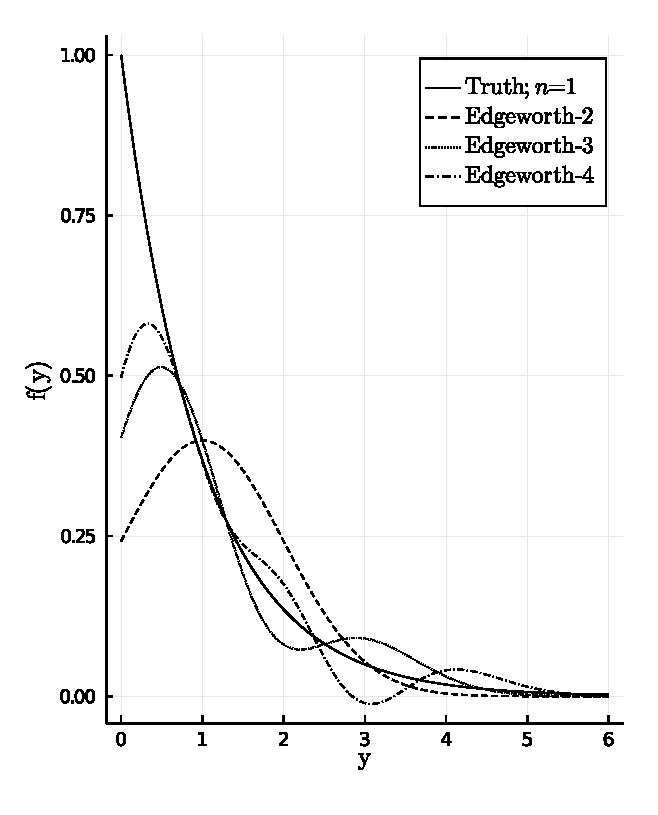
\includegraphics[width=8cm]{edgeworth_gamma11_1_terms.eps} 
        }
        \subfloat[$p=2; n=1$ \label{fig-single-gamma21}]{
            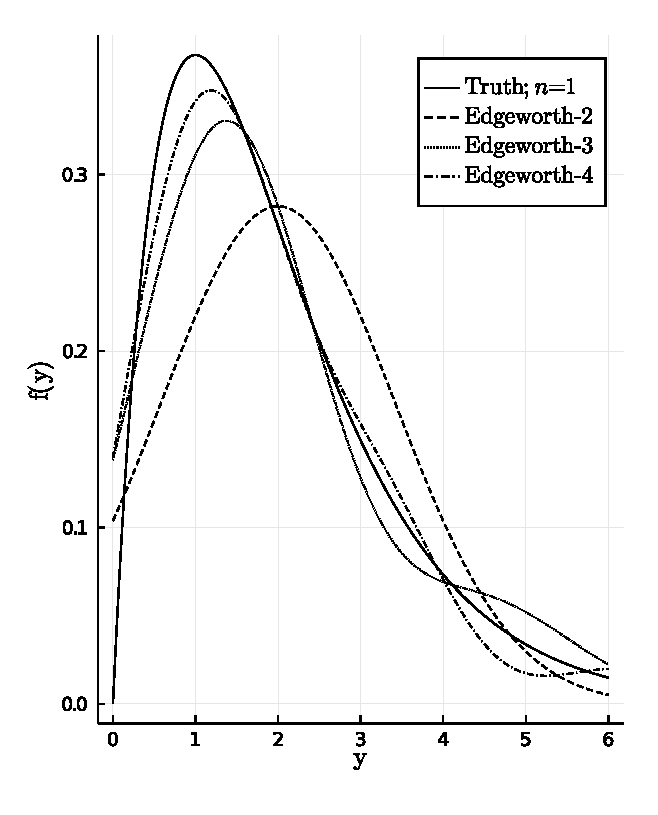
\includegraphics[width=8cm]{edgeworth_gamma21_1_terms.eps}
        }
        \qquad
        \subfloat[$p=1; n=10$ \label{fig-10-gamma11}]{
            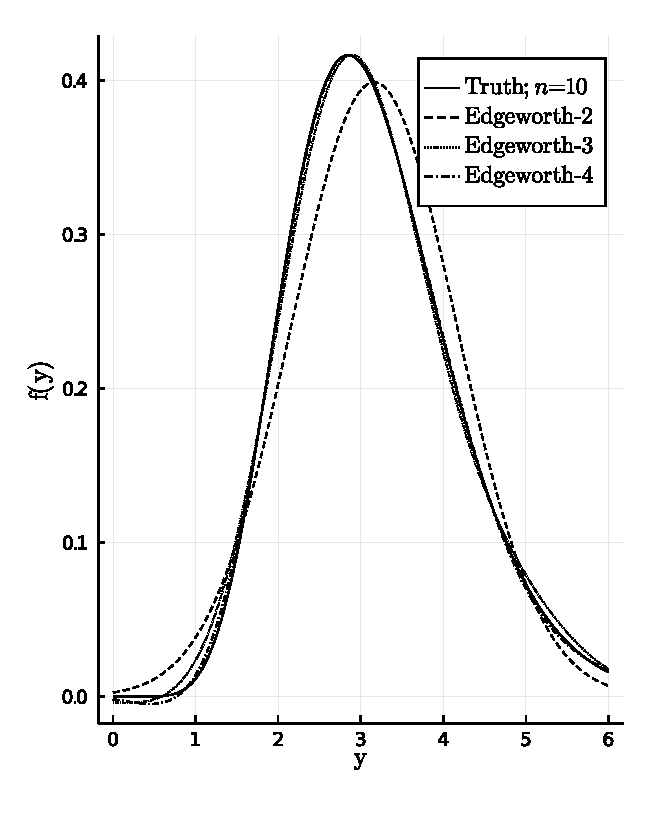
\includegraphics[width=8cm]{edgeworth_gamma11_10_terms.eps} 
        }
        \subfloat[$p=2; n=10$ \label{fig-10-gamma21}]{
            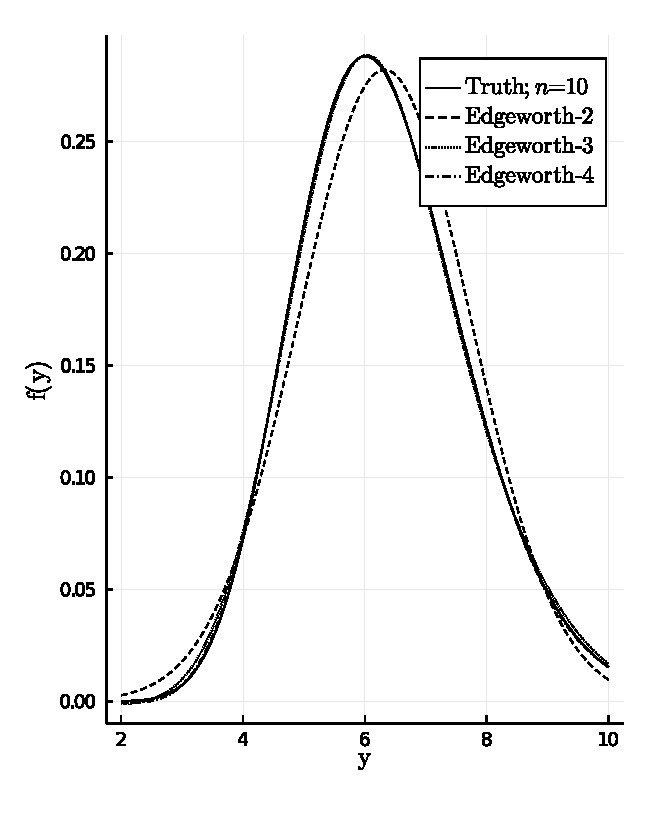
\includegraphics[width=8cm]{edgeworth_gamma21_10_terms.eps}
        }
        \caption{Several combinations of $p$ and $n$ exposing different behaviours of the Edgeworth approximation to the density of a standardized sum  of $n$ i.i.d.\,random variables following a $\Gamma(p, 1)$ distribution.}
        \label{fig-edgeworth}
    \end{figure}

    
    \begin{figure}[!htbp]
        \textbf{Approximation error of $\Gamma(p,1)$ standardized sums}
        \centering
        \subfloat[$p=1; n=1$\label{fig-err-abs-gamma11}]{
            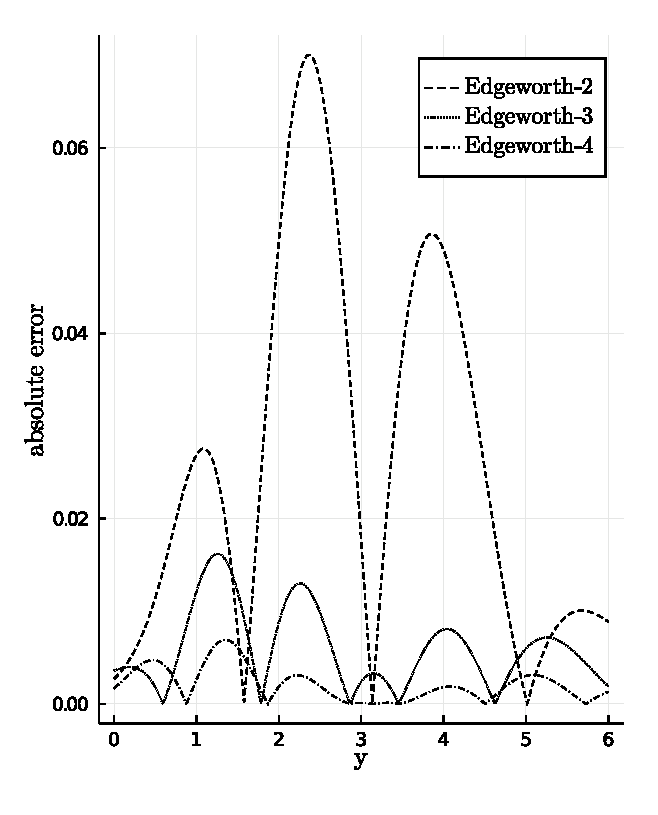
\includegraphics[width=7.5cm]{edgeworth_err_abs_gamma11_10_terms.eps} 
        }
        \subfloat[$p=2; n=1$ \label{fig-err-abs-gamma21}]{
            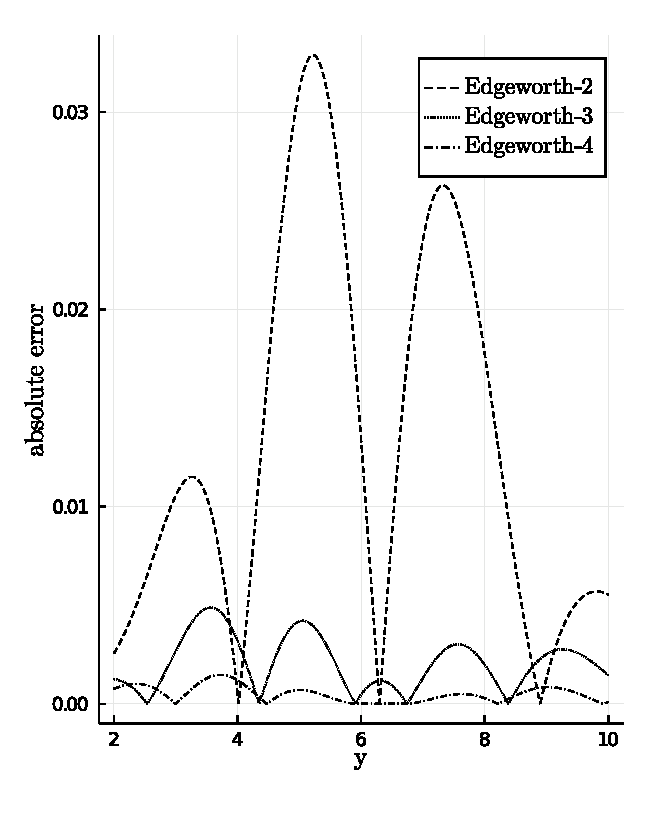
\includegraphics[width=7.5cm]{edgeworth_err_abs_gamma21_10_terms.eps} 
        }
        \qquad
        \subfloat[$p=1; n=10$ \label{fig-err-rel-gamma11}]{
            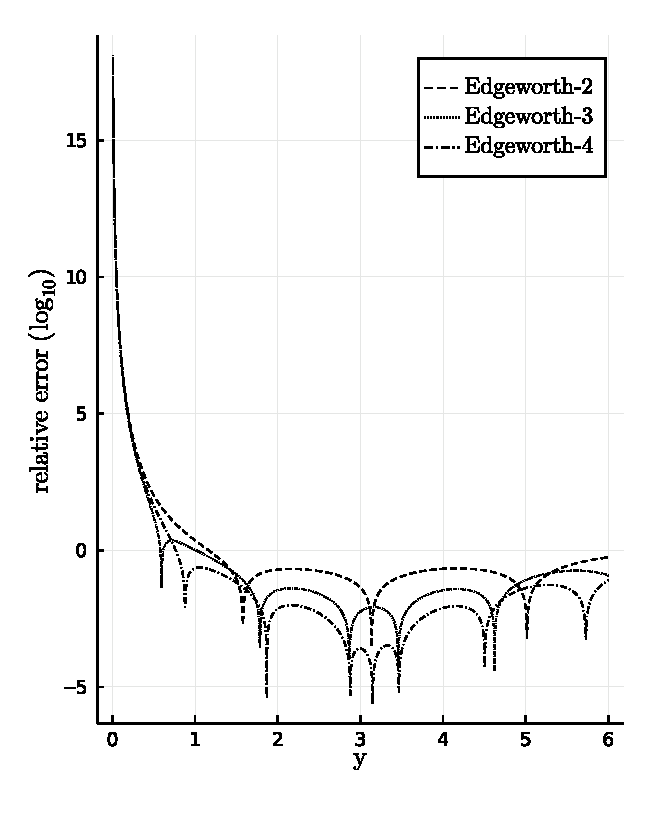
\includegraphics[width=7.5cm]{edgeworth_err_rel_gamma11_10_terms.eps}
        }
        \subfloat[$p=2; n=10$ \label{fig-err-rel-gamma21}]{
            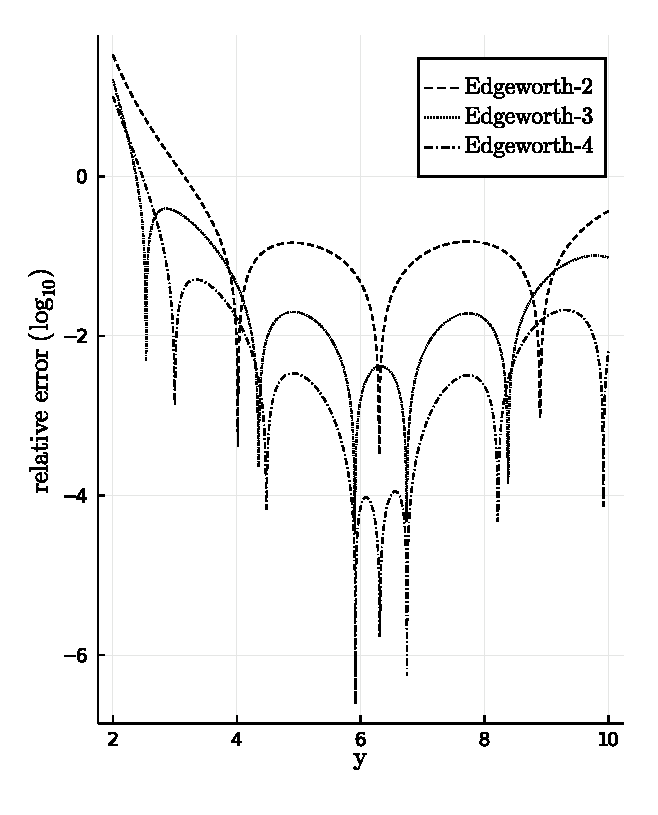
\includegraphics[width=7.5cm]{edgeworth_err_rel_gamma21_10_terms.eps}
        }
        \caption{Study of the approximation error of the Edgeworth approximation on a standardized sum of $n=10$ i.i.d.\,random variables following a $\Gamma(p, 1)$ distribution. The absolute error studied in Theorem \ref{thm-edgeworth} is well behaved as shown in the upper panel. However, the lower panel shows that the relative error of the approximation can be extremely high in low density regions where a low absolute error might still be a large relative error.}
        \label{fig-edgeworth-err}
    \end{figure}
    


    In Figure \ref{fig-edgeworth}, we show several examples of the behaviour of the Edgeworth approximation under different conditions. In the upper pane of Figure \ref{fig-edgeworth}, we compare the Edgeworth approximations of orders $k=2, 3, 4$ to the true density of a standardized sum of $n=1$ and $n=10$ random variables with a $\Gamma(p, 1)$ distribution for $p=1,2$. For $p=1$, $\Gamma(p, 1)$ is an exponential distribution. For $n = 1$, the discontinuity at $y = 0$ of the exponential distribution results in high oscillations of the Edgeworth approximation as demonstrated in Figure \ref{fig-single-gamma11} which even leads to negative values of the density approximation. Increasing to $p = 2$, we can see in Figure \ref{fig-single-gamma21} that the approximation is better behaved but unsurprisingly still does not well approximate the $\Gamma(2, 1)$ distribution. For both $p=1$ and $p=2$, increasing the number of terms summed to $n = 10$ results in seemingly good approximations to the density of the standardized sum as shown in Figures \ref{fig-10-gamma11} and \ref{fig-10-gamma21}.

    While Figure \ref{fig-edgeworth} appears to show good results of the Edgeworth approximation, it is hard to assess the quality of the approximations in regions of low probability. We display in Figure \ref{fig-edgeworth-err} the error of the Edgeworth series of orders $k=2,3,4$ approximating the density of a standardized sum of $n=10$ i.i.d.\,random variables following a $\Gamma(p, 1)$ distribution for $p=1$ and $p=2$. The upper pane demonstrates the control of the absolute approximation error studied in Theorem \ref{thm-edgeworth}. However, the lower panel of Figure \ref{fig-edgeworth-err} shows that the relative error can still reach very high values even as the order of the approximation increases. This is explained by the fact that even if the relative error is controlled, it might still be big relative to the true density in low probability regions.

    In many settings, one is interested in using distribution approximations to compute p-values in statistical tests. In this case, one is trying to find statistical evidence against a null hypotheses by demonstrating a low p-value of the null hypothesis model. Hence, the Edgeworth series itself can be ill suited for direct applications. However, as we will see in the next section, the Edgeworth approximation and related approximation results can still be used to construct approximations that are usable in to estimate the density function in low probability regions.
\end{example}

\subsection{Saddlepoint approximation} \label{sec-saddlepoint}

This section presents another approximation scheme based on the Edgeworth approximation, which resolves some of the issues of the Edgeworth approximation highlighted in the previous section.

We begin by introducing \textit{exponential tilting}. Consider a random variable $X \in \Rp$ with cumulant generative function $K$ and density $f$. We introduce the exponential family $\mathcal{T}_P = \{ P_\gamma \}_{\gamma \in \Rp}$ where each $P_\gamma \in \mathcal{T}_P$ is characterized by its density function $f(\cdot; \gamma)$ given by
\begin{equation*}
    f(x; \gamma) = f(x)\expf{\gamma^\top x - K(\gamma)}.
\end{equation*}
Note that by the definition of the cumulant generating function, $K(\gamma)$ is the right normalization factor for $f(\cdot; \gamma)$ to integrate to 1, and hence $f(\cdot; \gamma)$ is a valid density function. Furthermore, the original distribution $P$ is an element of $\mathcal{T}_P$ with $P = P_0$. Given two distributions $P_{\gamma_0}, P_\gamma \in \mathcal{T}_P$, their densities differ by a known factor
\begin{equation*}
    f(x; \gamma_0) = f(x; \gamma)\expf{(\gamma_0 - \gamma)^\top x - \left[K(\gamma_0) - K(\gamma)\right]}.
\end{equation*} 
Hence, choosing $\gamma_0 = 0$ gives $f(\cdot; \gamma_0) = f$ and the following holds for any $\gamma \in \Rp$
\begin{equation} \label{eq-saddlepoint-original}
    f(x) = f(x; \gamma)\expf{K(\gamma) - \gamma^\top x}.
\end{equation}
Therefore, we can construct an approximation of $f$ by choosing $\gamma$ such that $f(\cdot; \gamma)$ can be accurately approximated.

Let us now consider a distribution $P$ with cumulant generating function $K$. We wish to use the previous argumentation to approximate the density $f_n$ of the mean $S$ of $n$ i.i.d.\,random variables distributed according to $P$. Using that the cumulant generating function of $S$ is $K_n(t) = nK(t/n)$ and replacing it in (\ref{eq-saddlepoint-original}), we get
\begin{equation} \label{eq-fn-in-terms-of-fngamma}
    f_n(s) = f_n(s; \gamma)\expf{nK(\gamma / n) - \gamma^\top s},
\end{equation}
where $f_n(\cdot; \gamma)$ is the density of the mean of $n$ i.i.d.\,random variables distributed according to $P_\gamma$. Since the Edgeworth approximation was derived for a standardized sum of random variables, we apply the transformation
\begin{align*}
    \frac{1}{n}\sum_{i=1}^n X_i &\mapsto \frac{1}{\sqrt{n}}\sum_{i=1}^n \Sigma_\gamma^{-1/2}(X_i - \mu_\gamma)\\
    s &\mapsto s^* := \sqrt{n}\Sigma_\gamma^{-1/2}(s - \mu_\gamma)
\end{align*}
where $\mu_\gamma$ and respectively $\Sigma_\gamma$ are the mean and covariance under the distribution $P_\gamma$. Furthermore, the determinant of the transformation is $n^{p/2}|\Sigma_\gamma|^{-1/2}$, which gives, using the notation in (\ref{eq-edge-polynomial}),
\begin{equation} \label{eq-saddlepoint-poly}
    f_n(s; \gamma) = n^{p/2}|\Sigma_\gamma|^{-1/2} \phi(s^*)\left\{ 1 + P_{k, n}(s^*; \kappa(\gamma)) + o(n^{1-k/2})\right\},
\end{equation}
where $\kappa(\gamma)$ are the cumulants of the random variable distributed according to $P_\gamma$. The cumulant generating function $K(\cdot; \gamma)$ of $P_\gamma$ can be expressed in terms of the cumulant generating function $K$ by
\begin{equation*}
    K(t; \gamma) = K(t + \gamma) - K(\gamma).
\end{equation*}
Since the covariance matrix $\Sigma_\gamma$ is equal to the Hessian of the cumulant generating function $K(\cdot; \gamma)$ of $P_\gamma$ evaluated at 0, we have $\Sigma_\gamma = K''(\gamma)$. This lets us rewrite (\ref{eq-saddlepoint-poly}) in terms of $K$ as follows,
\begin{equation*}
    f_n(s; \gamma) = n^{p/2}|K''(\gamma)|^{-1/2} \phi(s^*)\left\{ 1 + P_{k, n}(s^*; \kappa(\gamma)) + o(n^{1-k/2})\right\}.
\end{equation*}

We are now interested in choosing $\gamma$ such that the Edgeworth approximation of $f_n(\cdot; \gamma)$ is accurate. As seen in Remark \ref{rem-edge-mean}, the third order Edgeworth approximation of even order has an error of order $o(n^{-2})$ instead of $o(n^{-3/2})$ when evaluated at the mean of the distribution. In other words, the Edgeworth approximation will be more accurate if $s^* = 0$ in the previous equation. Since $\gamma$ can be chosen freely and differently for each value $s$ at which the density $f_n$ is evaluated, we can choose $\gamma$ such that $s^* = 0$, or equivalently, such that $s = \mu_\gamma$. Similarly to the covariance matrix, we can write the mean of $P_\gamma$ as $\mu_\gamma = K'(\gamma)$. Hence, for any $s \in \Rp$, we find a distribution $P_{\hat\gamma_s} \in \mathcal{T}_P$ with mean $s$ by solving
\begin{equation} \label{eq-saddlepoint}
    K'(\hat\gamma_s) = s.
\end{equation}
We call the solution of this equation $\hat\gamma_s$ to emphasize the fact for each $s \in \Rp$, a different tilting distribution $P_{\hat\gamma_s}$ is chosen such that the Edgeworth approximation to the density of $P_{\hat\gamma_s}$ is accurate in $s$. Note that if $\hat\gamma_s$ solves (\ref{eq-saddlepoint}), it is also the maximum likelihood estimator of $\gamma$ within the model $\mathcal{T}_P$. Replacing $\gamma$ by $\hat\gamma_{s}$ in (\ref{eq-saddlepoint-poly}), we get
\begin{equation*}
    f_n(s; \hat\gamma_s) = \left(\frac{n}{2\pi}\right)^{p/2}|\Sigma_{\hat\gamma_s}|^{-1/2}\left\{ 1 + P_{k, n}(0; \kappa(\hat\gamma_s)) + o(n^{\floor{1-k/2}})\right\}.
\end{equation*}
Replacing $f_n(s; \gamma)$ by the approximation above in (\ref{eq-fn-in-terms-of-fngamma}) gives
\begin{align}
    f_n(s) &= \left(\frac{n}{2\pi}\right)^{p/2} \frac{\expf{nK(\hat\gamma_s / n) - \hat\gamma_s^\top s}}{|K''(\hat\gamma_s)|^{1/2}}  \left[1 + P_{k, n}(0; \kappa(\hat\gamma_s)) + o(n^{\floor{1-k/2}})\right]\nonumber\\
    &= g(s; K)\left[1 + P_{k, n}(0; \kappa(\hat\gamma_s)) + o(n^{\floor{1-k/2}})\right] \label{eq-saddle-exp}
\end{align}
where
\begin{equation*}
    g(s; K) = \left(\frac{n}{2\pi}\right)^{p/2} \frac{\expf{nK(\hat\gamma_s / n) - \hat\gamma_s^\top s}}{|K''(\hat\gamma_s)|^{1/2}}.
\end{equation*}
We call $g(\cdot; K)$ the \textit{Saddlepoint approximation} to the density of $S$. We now justify the approximation accuracy claim from (\ref{eq-saddle-exp}) in the following theorem.

\begin{theorem}
    Let $P$ be a distribution with cumulant genrating function $K$ and $k \in \N_{\geq 2}$ such that all cumulants of $P$ of order up to $k$ exist. Suppose that for every $s \in \Rp$, (\ref{eq-saddlepoint}) has a unique solution $\hat\gamma_s$. Let $n \in \N$ let $S$ be the mean of $X_1, \ldots, X_n \simiid P$,
    \begin{equation*}
        S = n^{-1} \sum_{i=1}^n X_i.
    \end{equation*}
    Then, if the density $f_n$ of $S$ exists, the expansion given in (\ref{eq-saddle-exp}) holds.
\end{theorem}
\begin{proof}
    This result is a direct consequence of Theorem \ref{thm-edgeworth}, applied pointwise to the tilted distribution $P_{\hat\gamma_s}$ for every $s \in \Rp$. As discussed above, Remark \ref{rem-edge-mean} implies that only powers of $n^{-1}$ have non-vanishing coefficients in the Edgeworth approximation of the tilted densities. This turn implies that the Edgeworth approximation error in each point is of order $o(n^{\floor{1-k/2)}})$, concluding the proof of the theorem.
\end{proof}

While the Saddlepoint approximation has many advantages over the Edgeworth approximation, it is important to note that the Saddlepoint approximation requires the complete cumulant generating function of the approximated density to be known. The Edgeworth approximation on the other hand only uses the first $k$ cumulants of the distributions, which are evaluations of derivatives of the cumulant generating function in 0. 

A special case of particular interest arrises when taking $k = 3$. In this case, the Edgeworth approximation of $f_n(\cdot; \hat\gamma_s)$ is equal to its normal approximation since the polynomial part $P_{k, n}(\cdot; \kappa(\hat\gamma_s))$ of $e_{k,n}(\cdot; \kappa(\hat\gamma_s))$ is equal to 0, giving
\begin{align} \label{eq-saddle-3}
    f_n(s) &= g(s; K)\left[1 + o(n^{-2})\right]\nonumber\\
    &= \left(\frac{n}{2\pi}\right)^{p/2} \frac{\expf{nK(\hat\gamma_s / n) - \hat\gamma_s^\top s}}{|K''(\hat\gamma_s)|^{1/2}} \left[1 + o(n^{-2})\right]
\end{align}
The Saddlepoint approximation of second order is commonly used in applications since it presents many advantages compared to the Edgeworth approximation. It has a simple expression which makes it easier to construct and manipulate it. Furthermore, the Saddlepoint approximation is often highly accurate or even exact up to normalization, and, unlike the other approximations presented so far, is always positive.

\begin{example} \label{ex-gamma-saddle}
    Extending Example \ref{ex-gamma-edge}, we analyze the behaviour of the Saddlepoint approximation to the mean $Y = n^{-1}\sum_{i=1}^n X_i \in \R_+$ where $X_1, \ldots, X_n \simiid \Gamma(p, \lambda)$. The cumulant generating function of the $\Gamma(n, p)$ distribution is $K(t) = p\logf{\lambda} - p\logf{\lambda - t}$ and its first derivative is $K'(t) = p / (\lambda - t)$. For any $s \in \R_+$, the Saddlepoint $\hat\gamma_s$ is given by the solution to the Saddlepoint Equation in (\ref{eq-saddlepoint}), which here becomes
    \begin{equation*}
        \frac{p}{\lambda - \hat\gamma_s/n} = s \Rightarrow \hat\gamma_s = n\left(\lambda - \frac{p}{s}\right).
    \end{equation*}

    \begin{figure}[!htbp]
        \textbf{Approximation error of $\Gamma(2,1)$ standardized sums with $n=10$}
        \centering
        \subfloat{
            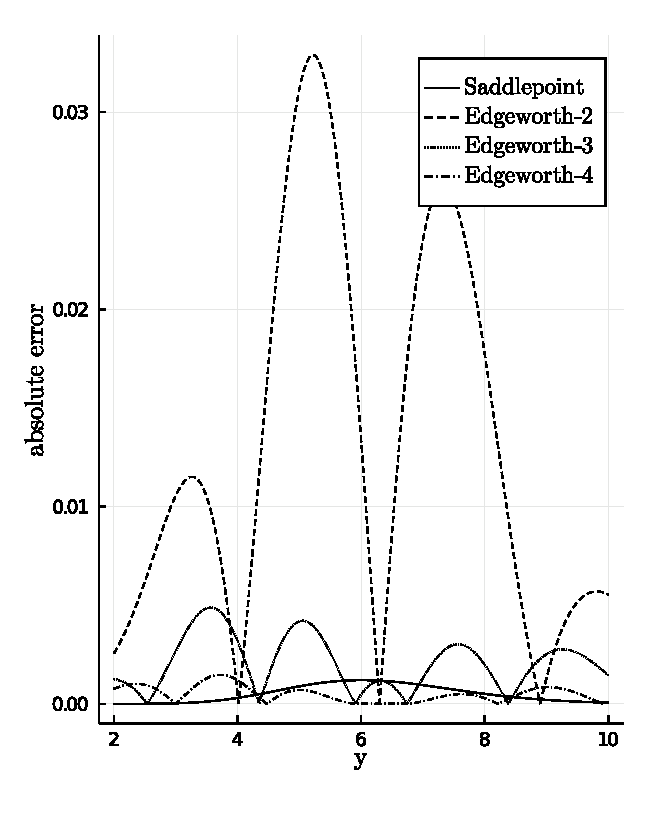
\includegraphics[width=7.5cm]{saddlepoint_and_edgeworth_err_abs_gamma21_10_terms.eps} 
        }
        \subfloat{
            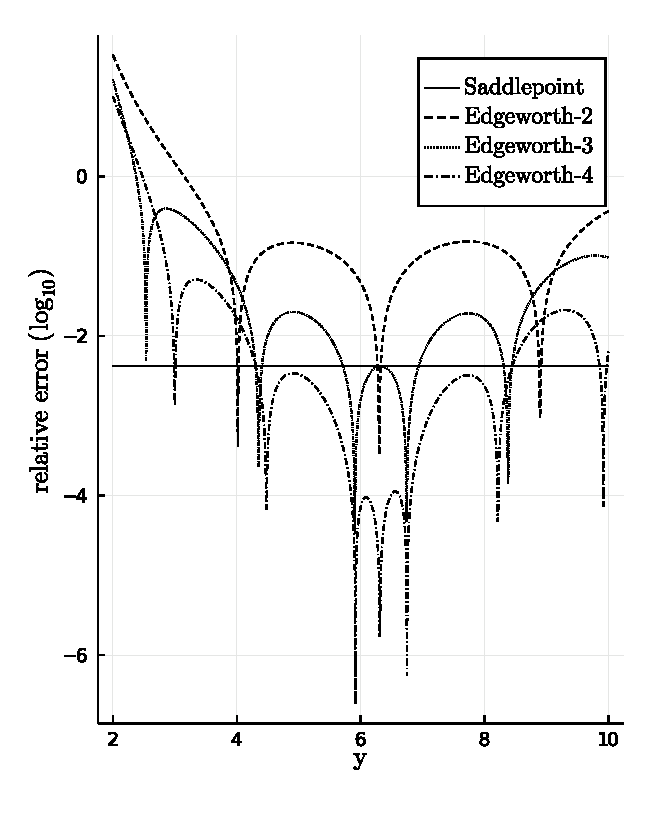
\includegraphics[width=7.5cm]{saddlepoint_and_edgeworth_err_rel_gamma21_10_terms.eps} 
        }
        \caption{Study of the error of the Saddlepoint approximation on a standardized sum $n=10$ i.i.d.\,random variables distributed according to $\Gamma(2, 1)$. Both panes demonstrate the properties studied of the Saddlepoint approximation: the accurate relative error, the gain in order of approximation and the uniform relative error of the approximation for sums of Gamma random variables.}
        \label{fig-saddlepoint-err}
    \end{figure}

    In Figure \ref{fig-saddlepoint-err}, we demonstrate how the Saddlepoint approximation of order 3 compares to the Edgeworth approximation when approximating a standardized sum of $n$ random variables independently distributed according to $\Gamma(2, 1)$. Since the standardized sum can be obtained by multiplying the mean by a factor of $\sqrt{n}$, the Saddlepoint approximation is easily adapted by change of variable. Both panels show accurate approximation properties both in terms of relative and absolute error.
    \newline
    In this example, it is also interesting to examine the explicit form of the Saddlepoint approximation $g$. Replacing the relevant quantities in (\ref{eq-saddle-3}), we obtain that the Saddlepoint approximation is
    \begin{align*}
        g(s; K) &= \sqrt{\frac{n}{2\pi K''(\lambda - \frac{p}{s})}} \expf{nK\left(\lambda - \frac{p}{s}\right) - n\left(\lambda - \frac{p}{s}\right)s}\\
        &= \sqrt{\frac{n}{2\pi s^2/p}} \expf{n\left(p\logf{\lambda} - p\logf{p/s}\right) - ns\lambda + np}\\
        &= (n\lambda)^{np}s^{np-1}\expf{-sn\lambda}  \frac{(np)^{1/2-np}\expf{np}}{\sqrt{2\pi}}.
    \end{align*}
    Consider now Stirling's formula for the gamma function
    \begin{equation*}
        \Gamma(z) \approx \sqrt{2\pi}z^{z-1/2}\expf{-z}.
    \end{equation*}
    We recognize that the second term in the expression of $g(s; K)$ corresponds to the inverse of Stirling's approximation of $\Gamma(np)$. Therefore, the Saddlepoint approximation to the density of the mean $n$ i.i.d.\,random variables distributed according to $\Gamma(p, \lambda)$ corresponds to the density of the true distribution $\Gamma(np, n\lambda)$ of the mean, where the gamma function has been replaced by Stirling's approximation. This has the interesting consequence that the relative error of the Saddlepoint approximation does not depend on $s$, the point at which the density is evaluated, but rather only depends on $n$. This behaviour is also seen in Figure \ref{fig-saddlepoint-err} where the relative error of the Saddlepoint approximation is a straight horizontal line. Daniels \cite{daniels1954saddlepoint} characterizes the class of distributions for which the uniform relative approximation error holds.

  
    
\end{example}

\subsection{The $p^*$ approximation in exponential families} \label{sec-pstar}

Next, we apply the Saddlepoint approximation to an exponential family $\mathcal{P} = \left\{P_\theta\right\}_{\theta}$ with natural parameter $\theta \in \Rp$. We write $f(\cdot; \theta)$ for the density of $P_\theta \in \mathcal{P}$. Then, $f(\cdot; \theta)$ is given by
\begin{equation*}
    f(x; \theta) = \expf{\theta^\top T(x) - \mathcal{H}(\theta) - \mathcal{G}(x)}.
\end{equation*}
Given a random sample $x = (x_1, \ldots, x_n)$ of $P_\theta$, the \textit{log-likelihood function} denoted $\ell(\cdot; x)$ is given by
\begin{equation*}
    \ell(\theta; x) = \theta^\top \sum_{i=1}^n T(x_i) - n \mathcal{H}(\theta) = n\left[\bar t - \mathcal{H}(\theta)\right],
\end{equation*}
where $\bar t = n^{-1}\sum_{i=1}^n T(x_i)$ is the sample average of the sufficient statistic. Hence, the maximum likelihood estimator of $\theta$ is the value $\hat\theta_{\bar t} \in \Rp$ satisfying the score equation
\begin{equation} \label{eq-score-expfam}
    \mathcal{H}'(\hat\theta_{\bar t}) = \bar t.
\end{equation}
For simplicity, we assume that $\mathcal{H}'$ is one-to-one to ensure that (\ref{eq-score-expfam}) has a unique solution $\hat\theta_{\bar t}$. In the exponential family $\mathcal{P}$, it can be shown that the cumulant generating function of any member $P_\theta \in \mathcal{P}$ is given by $K_\theta(t) = \mathcal{H}(\theta + t) - \mathcal{H}(\theta)$. Thus $K'_\theta(t) = \mathcal{H}'(\theta + t)$. Using the cumulant generating function in the score equation (\ref{eq-score-expfam}) gives
\begin{equation*}
    K'_\theta(\hat\theta_{\bar t} - \theta) = \bar t.
\end{equation*}
Consider the Saddlepoint equation given in (\ref{eq-saddlepoint}), and notice that the parameter $\hat\gamma_{\bar t}$ of the tilted family is related to the maximum likelihood estimator $\hat\theta$ by
\begin{equation*}
    \hat\gamma_{\bar t}/n = \hat\theta_{\bar t} - \theta.
\end{equation*}
Using this in the Saddlepoint approximation (\ref{eq-saddle-3}), we obtain that the Saddlepoint approximation for the average $\bar T = n^{-1}\sum_{i=1}^n T(X_i)$, where $X_1, \ldots, X_n \simiid P_\theta$, is
\begin{align*}
    g(\bar t; K_\theta) 
    &= \left(\frac{n}{2\pi}\right)^{p/2}|K_\theta''(\hat\theta_{\bar t} - \theta)|^{-1/2} \expf{nK_\theta(\hat\theta_{\bar t} - \theta) - (\hat\theta_{\bar t} - \theta)^\top \bar t}\\
    &= \left(\frac{n}{2\pi}\right)^{p/2}|\mathcal{H}''(\hat\theta_{\bar t})|^{-1/2} \expf{n(\mathcal{H}(\hat\theta_{\bar t}) - \mathcal{H}(\theta)) - (\hat\theta_{\bar t} - \theta)^\top \bar t}\\
    &= \left(\frac{n}{2\pi}\right)^{p/2}|j(\hat\theta_{\bar t})|^{-1/2} \expf{\ell(\theta; \bar t) - \ell(\hat\theta_{\bar t}; \bar t)},
\end{align*}
where the last equality follows from the fact that $\mathcal{H}''(\hat\theta)$ is equal to the observed Fisher information $j(\hat\theta)$. Daniels \cite{daniels1958} notes that this approximation can further be used to approximate the distribution of the maximum likelihood estimator. Let $\hat\Theta$ be the random variable solving the score equation $\mathcal{H}'(\hat\Theta) = \bar T$. By change of variable, we can use the approximation above to construct  the \textit{$p^*$ approximation} to the density of $\hat\Theta$, given by
\begin{equation*}
    p^*(\hat\theta; \theta, \bar t) = \left(\frac{n}{2\pi}\right)^{p/2}|j(\hat\theta)|^{-1/2} \expf{\ell(\theta; \bar t) - \ell(\hat\theta; \bar t)} \abs{\frac{\d \hat\theta}{\d \bar t}}^{-1}.
\end{equation*}
To compute the determinant of the Jacobian of the transformation $\hat\theta(\bar t)$, we  differentiate the score equation with respect to $\hat\theta$ to find $\mathcal{H}''(\hat\theta) = (\d \bar t / \d \hat\theta)$ and hence $(\d \hat\theta / \d \bar t) = \mathcal{H}''(\hat\theta)^{-1} = j(\hat\theta)^{-1}$. Therefore, the density of $\hat\Theta$ given the true parameter $\theta$ and the observation $\bar t$ is approximated by
\begin{equation} \label{eq-pstar}
    p^*(\hat\theta; \theta, \bar t) = \left(\frac{n}{2\pi}\right)^{p/2}|j(\hat\theta)|^{1/2} \expf{\ell(\theta; \bar t) - \ell(\hat\theta; \bar t)}.
\end{equation}
While the dependence on $\bar t$ naturally comes from the proposed derivation of the $p^*$ approximation, it is often more convenient to parametrize the loglikelihood $\ell(\cdot; x)$ and $p^*$ approximations in terms of the maximum likelihood estimator $\hat\theta(\bar t)$. We then write
\begin{equation*}
    p^*(\hat\theta; \theta, \hat\theta) = \left(\frac{n}{2\pi}\right)^{p/2}|j(\hat\theta)|^{1/2} \expf{\ell(\theta; \hat\theta) - \ell(\hat\theta; \hat\theta)}.
\end{equation*}
This highlights the fact that the $p^*$ approximation inherits its locality from the Saddlepoint approximation, since the density $p^*(\hat\theta; \theta, \hat\theta)$ is different at each point $\hat\theta$ at which it is evaluated. The $p^*$ approximation can also be used in many different situations where the distribution of refence is not necessarily an exponential family. Several articles and books by Barndorff-Nielsen\cite{BarndorffNielsen1980,BarndorffNielsen1983} and other authors study and derive the $p^*$ approximation in broader generality.

Suppose now that the exponential family $\mathcal{P}$ has an alternative parametrization $\{ P_\phi \}$ such that there exists a diffeomorphism $\phi = \phi(\theta)$ satisfying $\hat\phi = \phi(\hat\theta)$, where $\hat\phi$ and $\hat\theta$ are the maximum likelihood estimators in their respective parametrizations. Then, 
\begin{align*}
    p^*(\hat\phi; \phi, \hat \phi) 
&= \left(\frac{n}{2\pi}\right)^{-p/2}|j_\phi(\hat\phi)|^{1/2} \expf{\ell(\phi; \hat \phi) - \ell(\hat\phi; \hat \phi)}\\
&= \left(\frac{n}{2\pi}\right)^{-p/2}\left(|j_\theta(\theta(\hat\phi))|\abs{\frac{\d \hat\theta}{\d \hat\phi}}^{-2}\right)^{1/2} \expf{\ell(\theta(\phi); \theta(\hat \phi)) - \ell(\theta(\hat\phi); \theta(\hat \phi))}\\
&= p^*(\theta(\hat\phi); \theta(\phi), \theta(\hat \phi))\abs{\frac{\d \hat\theta}{\d \hat\phi}}^{-1}.
\end{align*}
Hence, the $p^*$ approximation is invariant under reparametrization. The next example demonstrates the use of the $p^*$ approximation and shows how the parameterization invariance can be useful when applying the approximation.

\begin{example}

    \begin{figure}[!htbp]
        \textbf{Error of $p^*$ approximation of MLE in $\t{Exp}(\lambda)$ model with $n=10$}
        \centering
        \subfloat{
            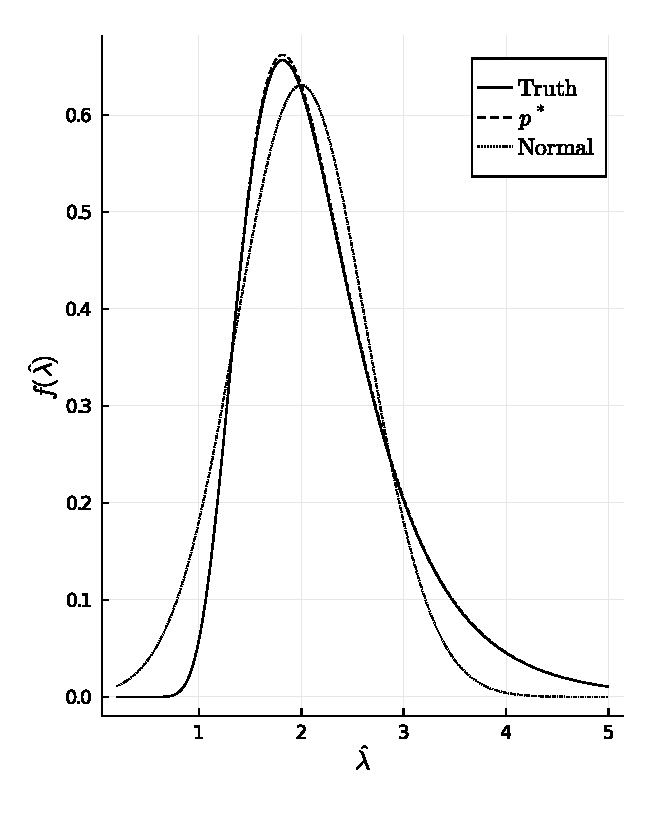
\includegraphics[width=8cm]{pstar_exp_dens.eps} 
        }
        \subfloat{
            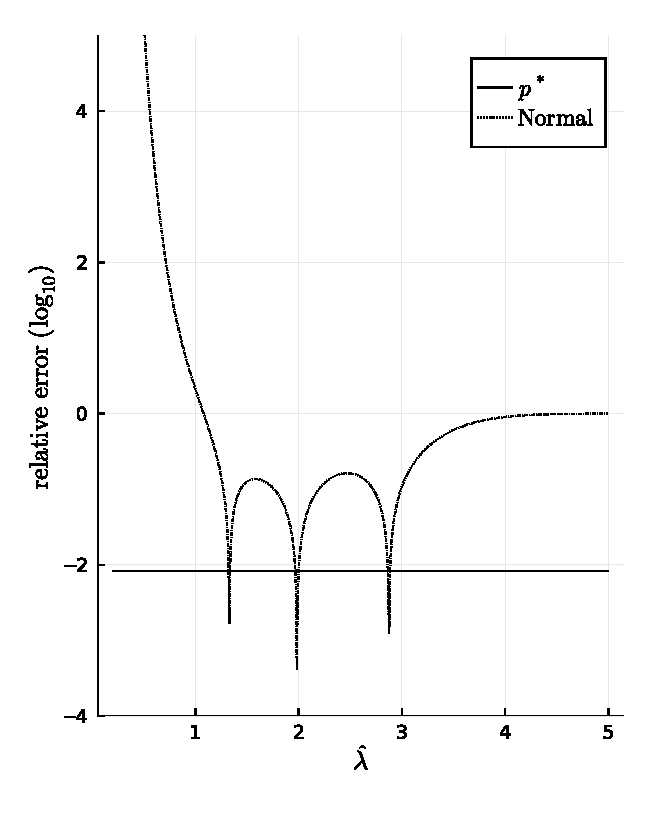
\includegraphics[width=8cm]{pstar_exp_err.eps} 
        }
        \caption{Study of the approximation error of the Saddlepoint approximation on a standardized sum of $n=10$ of $\Gamma(2, 1)$ random variables. Both panel exposes properties studied of the Saddlepoint approximation: the accurate rellative error, the gain in order of approximation and the uniform relative error of the approximation for sums of Gamma random variables.}
        \label{fig-pstar-approx}
    \end{figure}    

    We estimate the density of the maximum likelihood estimator of the parameter $\lambda \in \R_+$ of an exponential distribution $\t{Exp}(\lambda)$. The density of the distribution $\t{Exp}(\lambda)$ is
    \begin{equation*}
        f_\lambda(x) = \lambda \expf{-\lambda x}.
    \end{equation*}
    To make direct use of the $p^*$ approximation in (\ref{eq-pstar}), we must work in the natural parametrization of the exponential distribution. For $\lambda \in R_+$, the corresponding natural parameter is $\theta = -\lambda \in \R_-$ and the density of $\t{Exp}(\theta)$ is then $f_\theta(x) = \expf{ \theta x + \logf{-\theta}}$. Given an i.i.d.\,sample $x_1, \ldots, x_n$ of $\t{Exp}(\theta)$, the log-likelihood function is given by 
    \begin{equation*}
        \ell(\theta; \bar x) = n\left[\theta \bar x + \logf{-\theta}\right],
    \end{equation*}
    where we used that the sufficient statistic is $T(x) = x$ and hence $\bar t = \bar x$ is the sample mean. The maximum likelihood estimator of $\theta$ is then $\hat\theta = -1/\bar x$ and the observed information is equal to $j(\theta) = 1/\theta^2$.
    \\
    It follows that the $p^*$ approximation to the density of $\hat\theta$ is
    \begin{align*}
        p^*(\hat\theta; \theta, \hat\theta) 
        &= \sqrt{n} \frac{|\theta|^n}{|\hat\theta|^{n-1}}\expf{-n(\theta - \hat\theta)/\hat\theta} / \sqrt{2\pi}\\
        &= \sqrt{n} \frac{|\theta|^n}{|\hat\theta|^{n-1}}\expf{n\left[1 - \frac{\theta}{\hat\theta}\right]} / \sqrt{2\pi}.
    \end{align*}
    Using the invariance of the $p^*$ approximation, we obtain a $p^*$ approximation of the density of the maximum likelihood parameter $\hat\lambda$ in the original parametrization,
    \begin{align}
        p^*(\hat\lambda; \lambda, \hat\lambda) 
        &= p^*(\theta(\hat\lambda); \theta(\lambda), \theta(\hat\lambda)) \abs{\d \hat\theta / \d \hat\lambda}^{-1} \nonumber\\
        &= \sqrt{n} \frac{|\lambda|^n}{|\hat\lambda|^{n-1}}\expf{n\left[\frac{\lambda}{\hat\lambda} - 1\right]} / \sqrt{2\pi}. \label{eq-pstar-lambda}
    \end{align}
    
    The Normal approximation is a commonly used approximation to the distribution of the maximum likelihood estimator. In the exponential model, the Fisher information is $I(\lambda) = \lambda^{-2}$ and the following central limit theorem holds for the maximum likelihood estimator \cite[Example 3.12]{lehmann2006theory}
    \begin{equation} \label{eq-normal-lambda}
        \sqrt{n}(\hat\lambda - \lambda) \xrightarrow[]{\d} N(0, I(\lambda)^{-1})\ \ \ \  \t{as } n \rightarrow \infty.
    \end{equation}
    Hence, $\hat\lambda$ is approximately $N(\lambda, \lambda^2/n)$ with an approximation error of the density of $O(n^{-1/2})$. 
    
    In Figure \ref{fig-pstar-approx}, we display how (\ref{eq-pstar-lambda}) and (\ref{eq-normal-lambda}) approximate the density of $\hat\lambda$ under the true model $\t{Exp}(2)$. Since $\t{Exp}(\lambda) = \Gamma(1, \lambda)$, the distribution of $\bar X$ is $\Gamma(n, n\lambda)$ and hence $\hat\lambda = \bar x$ is $\t{Inv-}\Gamma(n, n\lambda)$. As we can see in the left panel, the $p^*$ approximation properly fits the true density of $\hat\lambda$ and captures the bias of the $\hat\lambda$ estimator as opposed to the Normal approximation which is centered around the true value of $\lambda$. Furthermore, we observe in the right panel how the relative error of the $p^*$ approximation is identical to the approximation error of the Saddlepoint approximation to the mean of $\Gamma(2, 1)$ seen in Example \ref{ex-gamma-saddle}. This is also a direct consequence of the invariance of the $p^*$ approximation since $\hat\Lambda$, the random variable associated to the maximum likelihood estimator, is the inverse of the sample mean $\bar X$, which is a diffeomorphic transformation for positive reals.
    

    \subsection{Julia implementation of higher-order approximations}
One is often confronted with challenges when translating mathematical ideas into executable software. Edgeworth series in particular are simple in their mathematical definition, but hide the use of many mathematical concepts that, independently, are commonly cumbersome to translate into easy-to-use and bug-free software. A generic implementation of Edgeworth series requires the ability to compute derivatives, express and manipulate asymptotic expansions and combine those to create density approximations.

Luckily, modern programming languages and libraries allow to quickly develop algorithms that are both efficient and close to their mathematical counterpart. In this thesis, we make use of the Julia programming language \cite{bezanson2017julia} and Julia bindings to the computer algebra system SymPy \cite{sympy}. The Julia programming language was chosen because it allows to write code that is generic enough to be used in various scenarios and extended with the ecosystem of libraries. For instance, one basic block of the approximations developed in this thesis is the cumulant generating function of a distribution. The cumulant generating function of a $\Gamma(\alpha, \beta)$ distribution can be defined as the function
\begin{lstlisting}[language=Julia, mathescape, escapechar=\%]
julia> gamma(p, $\lambda$) = t -> p*log($\lambda$) - p*log($\lambda$-t)
\end{lstlisting}
This function can then both be used with concrete values of $p, \lambda$ and $t$, for instance $\textrm{gamma}(1.0, 2.0)(1.0) = 0.6931471805599453$. However, one can also define symbolic variables for $p$ and $\lambda$ to construct a symbolic expression of the cumulant generating function
\begin{lstlisting}[language=Julia, mathescape, escapechar=\%]
julia> @syms p::positive $\lambda$::positive
julia> gamma(p, $\lambda$)(t)
p*log($\lambda$) - p*log($\lambda$-1.0)
\end{lstlisting}
This modularity can be used to construct helper functions to manipulate cumulant generating functions based on other libraries. For instance, if we are interested in computing the cumulants of a distribution, we can use the same definition of the cumulant function together and use the TaylorSeries \cite{TaylorSeries} library to efficiently compute the derivatives of the cumulant generating function. This let's us define the following function to compute the first $n$ cumulants of a distribution from its cumulant generating function
\begin{lstlisting}[language=Julia, mathescape, escapechar=\%, basicstyle=\small]
function cumulants(K, n; T=Number)
    t = Taylor1(T, n+1)
    (K(t).coeffs ./ exp(t).coeffs)[2:end]
end
\end{lstlisting}
Julia's extensibility makes it easy to combine several libraries to develop more advanced functionalities. For instace, we can the code presented above to compute the generic formula of the mean and variance of a $\Gamma(p, \lambda)$ distribution without having to program the interaction between Julia's SymPy bindings and the TaylorSeries library
\begin{lstlisting}[language=Julia, mathescape, escapechar=\%]
julia> @syms p::positive $\lambda$::positive
julia> $\mu,\ \sigma^2$ = cumulants(gamma(p, $\lambda$), 2)
2-element Vector{Sym}:
   p/$\lambda$
   p/$\lambda^2$
\end{lstlisting}
We used the capability of Julia to compose high-level libraries in order to develop a generic procedures for manipulating cumulant generating functions and develop density approximations for sums and maximum likelihood estimators. As an example, Listing \ref{lst-edgeworth} implements an arbitrary-order Edgeworth expansion by combining the mathematical derivation of the Edgeworth series in Section \note{TODO add ref} and some of the ideas described above.

A particularly appealing example of the usage of the function in Listing \ref{lst-edgeworth} is to derive the generic formula of the Edgeworth series of a specific order given the required cumulants. We start by defining a function \lstinline{symcgf(cumulants)} which creates a cumulant generating function with cumulants provided as an argument. For instance,
\begin{lstlisting}[language=Julia, mathescape, escapechar=\%]
julia> @syms t::real $\kappa_3$::real $\kappa_4$::real
julia> K = symcgf([0.0; 1.0; $\kappa_3$; $\kappa_4$])
julia> cumulants(K, 5; T=Sym)
5-element Vector{Sym}:
 0
 1
 $\kappa_3$
 $\kappa_4$
 0
\end{lstlisting}
We can then use the \lstinline{edgeworth} from Listing \ref{lst-edgeworth} to compute the explicit formula for the Edgeworth series of order 4\footnote{To avoid writing out the Hermite polynomials, we use a sligthly modified version of the code in Listing \ref{lst-edgeworth} replacing Hermite polynomials by symbolic functions $H_k$.}
\newpage
\begin{lstlisting}[language=Julia, mathescape, escapechar=\%]
julia> edgeworth(K, n, 4; T=Sym)(x)
                                                    -$x^2$  
                  /                             \   ---
                  |    $\kappa_3^2$$H_6$(x)      $\kappa_4H_4$(x)      $\kappa_3H_3$(x)     |   2  
0.398942280401433 |1 + ------ + ------ + ------- | e    %\footnote{This output was lightly adapted to properly render in LaTeX. }%
                  |     72n       24n     6$\sqrt{n}$      |      
                  \                             /    

\end{lstlisting}
With $(2\pi)^{-1/2} \approx 0.398942280401433$, this formula corresponds expression derived in Equation (\ref{eq-edgeworth-1d-4}) of Example \ref{ex-edgeworth-1d}.

\begin{lstlisting}[language=Julia, mathescape, escapechar=\%, caption={Symbolic implementation of the Edgeworth expansion}, label={lst-edgeworth}, basicstyle=\small]
function edgeworth(K, nsum, order; T=Float64)
    H(k) = basis(ChebyshevHermite, k)
    finaltype = promote_rule(T, typeof(nsum))
    taylororder = 3*order+1

    # Define two symbolic variables t and n. We use t as
    # variable  of the cgf for computing Taylor series and
    # n as the symbolic number of elements in the sum in
    # order to be able to track terms of various orders of n.
    @vars t n::(positive, integer)

    # Start by constructing the cgf of $\sum (X_i - \mu)/\sqrt{\sigma^2 n}$,
    # as discussed in Remark %\ref{rem-centering}%.
    $\mu$, $\sigma^2$ = cumulants(K, 2; T=T)
    stdK = affine(K, -$\mu$, 1/sqrt($\sigma^2$*n))
    sumK = iidsum(stdK, n)

    # Use the new cgf to construct the expansion of the ratio 
    # of characteristic functions, as in Equation (%\ref{eq-char-expansion}%).
    ratio = exp(sumK(t) - t^2/2)
    expansion = ratio.series(t, n=taylororder).removeO()

    # Then proceed by truncating the expansion to the desired 
    # order and replace the symbolic n by its true value.
    expansion = collect(expand(expansion), n)
    expansion = truncate_order(expansion, n, (1-order)/2)
    expansion = subs(expand(expansion), n, nsum)

    # The `expansion` variable is now a symbolic polynomial 
    # in the variable t. We retrieve the density by Fourier 
    # inversion, by which we replace instances of t^k by the 
    # k-th Hermite polynomial as in Equation (%\ref{eq-edgeworth-full}%).
    $\alpha$star = collect(expansion, t).coeff.(t.^(0:taylororder))
    $\alpha$star = convert.(finaltype, $\alpha$star)
    polynomial = sum([$\alpha$star[i]*H(i-1) for i=1:length($\alpha$star)])

    # Finally, the approximate density can be constructed
    # as done in %\ref{eq-edgeworth-full}% and using Remark %\ref{rem-centering}%.
    function density(z)
        $\kappa_1$ = sqrt(nsum)*$\mu$; x = (z - $\kappa_1$) / sqrt($\sigma^2$)
        return exp(-x^2/2)/sqrt($\sigma^2$*2$\pi$) * polynomial(x)
    end
end
\end{lstlisting}

\end{example}


% \section{The Edgeworth expansion}

% \chapter{The Barndorff-Nielsen formula in exponential families}

% \section{Tilted approximations in exponential families}

% \section{The $p^*$ formula}

% \section{Some applications of the $p^*$ formula}

\part{Gaussian Graphical Models}

\begin{itemize}
    \item clique, set of cliques
    \item chordal graph
    \item matrix indexing $A_C$ and $A_{C, C}$
    \item $A = M_{C, D}$ submatrix, then $[A]^\Gamma$ is $|\Gamma| \times |\Gamma|$ equal to $A$ on $\eset{C, D}$ and 0 otherwise.
\end{itemize}


\subsection{MLE in Gaussian graphical models}

A graphical model is a probabilistic models associating relations between random variables to a graph. The random variables of the model are represented by nodes in the graph and conditional independence relations are represented by missing edges between the corresponding nodes of the graph.

Consider a random vector $X$ distributed according to the \textit{multivariate Gaussian} distribution $N_p(0, \Omega^{-1})$ where $\Omega \in \S^p_{\succ 0}$ is the inverse of the \textit{covariance matrix} $\Sigma$ and is called the \textit{precision matrix}. The density of $X$ is then
\begin{equation} \label{eq-density-gaussian}
    f(x; \Omega) = (2\pi)^{-p/2} |\Omega|^{1/2} \expfc{-\frac{1}{2} \trB{xx^\top \Omega} }.
\end{equation}
We clearly see that the multivariate Gaussian distribution is an exponential family with canonical parameter $\Omega$ and sufficient statistic $\frac{1}{2}xx^\top$. 

We choose to parametrize the multivariate Normal distribution in terms of the precision matrix because of its special role in the context of graphical models. Indeed, the conditional independence relations of the entries a random vector $X \sim N_p(0, \Omega)$ are characterized by the sparsity patterns of the precision matrix $\Omega$.
\
\begin{lemma}
    Let $X \sim N_p(\mu, \Sigma)$ and let $i, j \in [p]$, then
    \begin{equation*}
        \Omega_{ij} = 0 \iff X_i \independent X_j | X_{[p] \setminus \eset{i,j}}.
    \end{equation*}
\end{lemma}
\begin{proof}
    By Lemma \ref{lem-gaussian-cond}, we have that the bivariate vector $X_{\eset{i,j}}$ is Gaussian with covariance matrix $\Sigma_{\eset{i,j}|[p]\setminus\eset{i,j}}$ equal to the Schur complement of $\Sigma_{[p] \setminus \eset{i,j}}$. The claim of this lemma is thus equivalent to 
    \begin{equation*}
        \Omega_{ij} = 0 \iff \Sigma_{\eset{i,j}|[p]\setminus\eset{i,j}}\ \t{is diagonal}.
    \end{equation*}
    Using the Schur complement inverse property, we have 
    \begin{equation*}
        \Sigma_{\eset{i,j}|[p]\setminus\eset{i,j}} 
        = \left[\Omega_{\eset{i,j}}\right]^{-1} 
        = \begin{pmatrix}
            \Omega_{ii} & \Omega_{ij}\\
            \Omega_{ji} & \Omega_{jj}
            \end{pmatrix}^{-1}
        = \frac{1}{|\Omega_{\eset{i,j}}|} \begin{pmatrix}
            \Omega_{jj} & -\Omega_{ij}\\
            -\Omega_{ji} & \Omega_{ii} 
            \end{pmatrix}^{-1}.
    \end{equation*}
    Hence, $\Sigma_{\eset{i,j}|[p]\setminus\eset{i,j}}$ is diagonal if and only if $\Omega_{ij} = 0$.
\end{proof}

Consider a graph $\G = ([p], E)$. We say that $X$ satisfies the \textit{Gaussian graphical model} with graph $\G$ if $X \sim N_p(0, \Omega)$ and
\begin{equation} \label{eq-ggm}
    \Omega_{i j} = 0 \iff \eset{i,j} \notin E.
\end{equation}
This property corresponds to the pairwise Markov property in graphical model theory. All together, we find that the independence relations of the entries of $X$, the connectivity of the nodes in $\G$ and the sparsity pattern of $\Omega$ are all the same concept viewed from a different angle which each on its own will help in studying them.

We now study properties of the maximum likelihood estimator in a Gaussian graphical model, largely following the presentation of Uhler \cite[Section 9]{maathuis2018handbook}.

Consider now a sample $X = (X^{1}, \ldots, X^{n})$ from a Gaussian distribution. The log-likelihood function for a precision matrix $\Omega \in \S^p_{\succ 0}$ obtained from (\ref{eq-density-gaussian}) is
\begin{equation*}
    \ell(\Omega; X) = \frac{n}{2} \log |\Omega| - \frac{1}{2}\tr[XX^\top\Omega].
\end{equation*}
Rewriting it in terms of the sufficient statistic $S = n^{-1}XX^\top$, we have
\begin{equation} \label{eq-likelihood}
    \ell(\Omega; S) = \frac{n}{2}\log |\Omega| - \frac{n}{2}\tr[S\Omega].
\end{equation}
In the \textit{saturated model} where no constraints are put on the entries of $\Omega$, the maximum likelihood estimator is defined when $S \in S^p_{\succ 0}$ and is equal to
\begin{equation*}
    \hat\Omega = S^{-1}.
\end{equation*}
However, if we are interested in estimating the maximum likelihood estimator $\hat\Omega$ of a Gaussian graphical model with graph $\G = ([p], E)$, the solution $\hat\Omega$ must lie in the subset $\S(\G)$ of $\S^p_{\succ 0}$ in which the conditional independence relations encoded in $\G$ are satisfied. This subset is directly given by Equation (\ref{eq-ggm}), $\S(\G) = \{ \Omega \in \S^p_{\succ 0} : \Omega_{ij} = 0 \t{ if } i \neq j \t{ and } \eset{i,j} \notin E \}$. We are then left with the following optimization problem
\begin{align} \label{eq-primal}
    \begin{split}
        &\underset{\Omega \in \S^p_{\succ 0}}{\t{maximize}}\ \  \log |\Omega| - \tr[S\Omega]\\
        &\t{subject to}\ \ \Omega \in \S(\G).
    \end{split}
\end{align}
Since the Gaussian graphical model condition is a linear constraint, the set $\S(\G)$ is the is a convex cone. Showing that the objective function in (\ref{eq-primal}) is concave would imply that maximum likelihood estimation in Gaussian graphical models is a convex optimization problem which would allow us to bring new insights to the problem by studying its dual formulation. We start by proving that the objective function is indeed concave.
\begin{lemma}
    The function $f : \S^p_{\succ 0} \rightarrow \R, X \mapsto \log |X| - \trB{SX}$ is concave.
\end{lemma}
\begin{proof}
    Since the sum of a linear function and a concave function is concave, and $\trB{SX}$ is linear in $X$, it is sufficient to show that the logarithm of the determinant of a matrix is a concave function. To do this, let us consider the line $\eset{ U + tV : t \in \R }$ for $U, V \in \S^p_{\succ 0}$. We can show that $X \mapsto \log |X|$ is concave on $\S^p_{\succ 0}$ by showing that $g(t) = \log |U + tV|$ is concave. Since $U \in \S^p_{\succ 0}$, both $U^{1/2}$ and $U^{-1/2}$ exist and we have 
    \begin{align*}
        g(t)
        &= \log |U + tV| \\
        &= \log |U^{1/2}(1_p + tU^{-1/2}VU^{-1/2}|\\
        &= \log |U| + \log |1_p + tU^{-1/2}VU^{-1/2}|\\
        &= \log |U| + \sum_{i=1}^p \log (1 + t\lambda_i),
    \end{align*}
    where $\lambda_i$ are the eigenvalues of $U^{-1/2}VU^{-1/2}$ and we use that the eigenvalues of $1_p + tU^{-1/2}VU^{-1/2}$ are $1 + t\lambda_i$. Since each $\log (1 + t\lambda_i)$ is concave in $t$, we have that $g$ is concave, completing the proof.
\end{proof}

We can now study the dual problem to (\ref{eq-primal}). The Lagragian of the maximum likelihood estimation in Gaussian graphical models is
\begin{align*}
    \mathcal{L}(\Omega, \nu)
    &= \log |\Omega| - \tr[S\Omega] - 2 \sum_{\eset{i, j} \notin E} \nu_{ij}\Omega_{ij}\\
    &= \log |\Omega| - \sum_{i=1}^p S_{ii}\Omega_{ii} - 2 \sum_{\eset{i,j} \in E} S_{ij}\Omega_{ij} - 2 \sum_{\eset{i, j} \notin E} \nu_{ij}\Omega_{ij}
\end{align*}
The Lagrange dual $H$ of (\ref{eq-primal}) is given by $H(\nu) = \mathcal{L}(\Omega^\nu, \nu)$ where $\Omega^\nu$ is the maximizer of $\mathcal{L}(\Omega, \nu)$. Derivating the expression of $\mathcal{L}(\Omega, \nu)$, we get that the inverse $\Sigma^\nu$ of $\Omega^\nu$ satisfies
\begin{equation*}
    \Sigma^\nu_{ij} = \begin{cases}
        S_{ij}\ \t{ if } i = j \t{ or } \eset{i, j} \in E\\
        \nu_{ij}\ \t{otherwise}.
    \end{cases}
\end{equation*}
Note that $\Sigma^\nu$ is the matrix formed by replcing entries in $S$ corresponding to missing edges with entries of the dual variables $\nu_{ij}$. Replacing this in the expression for the Lagrange dual function $H$, we obain
\begin{align*}
    H(\nu) 
    &= \log |\Omega^\nu| - \tr[S\Omega^\nu] - 2 \sum_{\eset{i, j} \notin E} \nu_{ij}\Omega^\nu_{ij}\\
    &= \log |\Omega^\nu| - \tr[\Sigma^\nu\Omega^\nu] + 2 \sum_{\eset{i, j} \notin E} \Sigma^\nu_{ij}\Omega^\nu_{ij} - 2 \sum_{\eset{i, j} \notin E} \nu_{ij}\Omega^\nu_{ij}\\
    &= \log |\Omega^\nu| - p = -\log |\Sigma^\nu| - p.
\end{align*}
And hence the dual to (\ref{eq-primal}) is
\begin{align} \label{eq-dual}
    \begin{split}
        &\underset{\Sigma \in \S^p_{\succ 0}}{\t{minimize}}\ \  -\log |\Sigma| - p\\
        &\t{subject to}\ \ \Sigma_{ij} = S_{ij}\ \t{ for all } i = j \t{ or } \eset{i, j} \in E
    \end{split}
\end{align}
To show that we can equivalently study problem (\ref{eq-primal}) and (\ref{eq-dual}), we must show that strong duality holds for this convex optimization problem. By \textit{Slater's constraint quantification} \cite[Section 5.3.2]{boyd2004convex}, it is enough to show that there exists an $\Omega^* \in \S^p_{\succ 0}$ that is strictly feasable for the primal problem. Since the identity matrix is positive definite and is an element of $\S(\G)$ for any $\G$, strong duality holds for any graph $\G$ and we can freely study both formulations of the optimization problem. Furthermore, problems (\ref{eq-primal}) and (\ref{eq-dual}) have a solution if and only if $\log |\Sigma| + p$ is unbounded from above in the set of feasable matrices. We have yet to study under which condition this is the case.

To that end, let us first introduce some new notation. If $\G$ is a graph over $p$ nodes and $\Sigma \in \R^{p\times p}$, the $\G$-partial matrix $\Sigma^\G$ of $\Sigma$ is the partial matrix found by removing entries in $\Sigma$ corresponding to missing edges in $\G$, see Figure \ref{fig-no-completion} for an example.With this notation, we can reformulate the dual problem (\ref{eq-dual}) as
\begin{align} \label{eq-completion}
    \begin{split}    
        &\underset{\Sigma \in \S^p_{\succ 0}}{\t{minimize}}\ \  -\log |\Sigma| - p\\
        &\t{subject to}\ \ \Sigma^\G = S^\G.
    \end{split}
\end{align}
If this formulation, the dual optimization problem corresponds to a \textit{positive definite matrix completion} problem in which the matrix $\Sigma$ is partially specified from entries of the sample covariance matrix corresponding to edges present in $\G$. Furthermore, Uhler \cite[Section 9.4]{maathuis2018handbook} presents a geometric argument tying together the matrix completion approach to the problem to its original convex optimization formulation.

\begin{theorem}
    Consider a Gaussian graphical model associated to the graph $\G$ and a sample covariance matrix $S$. The maximum likelihood estimation problems have unique solutions $\hat\Omega$ and $\hat\Sigma$ if and only if $S^\G$ has a positive definite completion. In this case, $\hat\Sigma$ is the positive definite completion of $S^\G$ and $\hat\Omega = \hat\Sigma^{-1}$.
\end{theorem}
\begin{proof}
    This theorem is a reformulation of Theorem 9.4.2 in \cite{maathuis2018handbook} in which $\c{L} \cap \S^p_{\succ 0} = \S(\G)$ which we have shown to contain at least $1_p$.
\end{proof}

We can now study the existence of a solution to the maximum likelihood question by finding the conditions under which a $\G$-partial sample covariance matrix can be completed to a positive definite matrix. Gross et al.\,\cite{10.3150/16-BEJ881} introduce the \textit{maximum likelihood threshold} of a graph $\G$, denoted $\t{mlt}(\G)$. The maximum likelihood treshold of a graph $\G$ is the smallest number of data points that guarantees that the maximum likelihood estimator exist almost surely in a Gaussian graphical model associated to the graph $\G$. In other words, $\t{mlt}(\G)$ is the smallest number of observations for which $S^\G$ can be completed to a positive definite matrix. For a Gaussian graphical model over $p$ variables, the rank of the sample covariance constructed from a sample of $n$ observations is $\t{rank}(S) = \min(n, p)$. Hence, if $n \geq p$, $S$ itself is a valid positive completing for $S^\G$, giving the worst case bound
\begin{equation} \label{eq-pessimistic-mlt}
    \t{mlt}(\G) \leq p,
\end{equation}
where equality holds if $\G$ is complete.

A necessary condition for a solution to the matrix completion problem to exist is that all completely specified principal submatrices $S^\G_{[p]\setminus I}$ of $S^\G$ for $I \subset [p]$ must be positive definite. The principal submatrix $S^\G_{[p]\setminus I}$ of $S^\G$ is completely specified if it contains no missing value. The necessary condition can be easily shown with the following argument: let $S^\G_{[p]\setminus I}$ be a principal completely specified submatrix of $S^\G$ such that there exists a $z \in \R^{p-|I|}\setminus \eset{0}$ with $z^\top S^\G_{-I} z \leq 0$. Then if $S^\G_+$ is the positive definite completion of $S^\G$, it holds that $x^\top S^\G_+ x \leq 0$ for $x \in \R^p \setminus \eset{0}$ with $x_I = z$ and $x_{-I} = 0$, contradicting the positive definiteness of $S^\G_+$. Furthermore, if $C$ is a clique of $\G$, $C$ is complete and thus the submatrix $S^\G_C$ is a completely specified principal submatrix of $S^\G$. Since $S^\G_C$ is complete, it is positive definite with probability one if and only if $n \geq |C|$. With $q(\G) = \max \eset{|C| : C \t{ is a clique of } \G}$ the maximum clique size in $\G$, we can lower bound the maximum likelihood threshold
\begin{equation*}
    q(\G) \leq \t{mlt}(\G).
\end{equation*}


\begin{figure}[!tbp]
    \begin{minipage}[c]{.3\linewidth}
        \centering
        \begin{gather*}
            \begin{pmatrix}
                1 & 0.9 & 0.3 & -0.9 \\
                0.9 & 1 & 0.9 & -0.7 \\
                0.3 & 0.9 & 1 & 0.9 \\
                -0.9 & -0.7 & 0.9 & 1
            \end{pmatrix}\\
            S
        \end{gather*}
    \end{minipage}
    \hfill
    \begin{minipage}[c]{.2\linewidth}
        \centering
        \begin{tikzpicture}[node distance={15mm}, thick, main/.style = {draw, circle}] 
            \node[main] (1) {$x_1$}; 
            \node[main] (2) [below left of=1] {$x_2$};
            \node[main] (3) [below right of=2] {$x_3$}; 
            \node[main] (4) [above right of=3] {$x_4$};
            \draw (1) -- (2);
            \draw (2) -- (3);
            \draw (4) -- (3);
            \draw (1) -- (4);
        \end{tikzpicture}
    \end{minipage}
    \hfill
    \begin{minipage}[c]{.3\linewidth} %inequalities
        \centering
        \begin{gather*}
             \begin{pmatrix}
                1 & 0.9 & ? & -0.9 \\
                0.9 & 1 & 0.9 & ? \\
                ? & 0.9 & 1 & 0.9 \\
                -0.9 & ? & 0.9 & 1
            \end{pmatrix}\\
            S^\G
        \end{gather*}
    \end{minipage}

    \caption{Example from \cite[Section 9.3]{maathuis2018handbook} of a matrix $S$ for which all completely specified submatrices of $S^\G$ are positive definite but which doesn't have a positive definite completion.}
    \label{fig-no-completion}
\end{figure}

However, as shown in the Example in Figure \ref{fig-no-completion}, this condition is not sufficient for the existence of a positive definite completion. Still, Grone et al. \cite{GRONE1984109} show that this condition is also sufficient exactly for chordal graphs.
\begin{theorem} \label{thm-chordal-iff}
    For a graph $\G$, the following statements are equivalent
    \begin{itemize}
        \item[(a)] A partial matrix $M^\G$ has a positive definite completion if and only if all completely specified submatrices of $M^\G$ are positive definite.
        \item[(b)] $\G$ is chordal.
    \end{itemize}
\end{theorem}
A consequence of this theorem is that if $\G$ is a chordal graph, $\t{mlt}(\G) = q(\G)$. This result for chordal graphs can be used to compute an upper bound on the maximum likelihood treshold of a general graph tighter than the worst-case one in (\ref{eq-pessimistic-mlt}). 

Let $\G = (\Gamma, E)$ be a graph and $S$ a sample covariance matrix. A graph $\G^+ = (\Gamma, E^+)$ is called a \textit{chordal cover} of $\G$ if $E \subset E^+$ and $\G^+$ is chordal. Then, since $E \subset E^+$, we have that the $\G^+$-partial matrix $S^{\G^+}$ agrees with the $\G$-partial matrix $S^\G$ on the entries corresponding to the edges $E$ of $\G$. Thus, one can view $S^{\G^+}$ as a partial completion of $S^\G$ and any positive definite completion of $S^{\G^+}$ is a valid positive completion of $S^\G$. Together with Theorem \ref{thm-chordal-iff} to show the following bound
\begin{equation*}
    \t{mlt}(\G) \leq q^+(\G) = \min \eset{ q(\G^+) : \G^+ \t{ is a chordal cover of } \G },
\end{equation*}
anda all together for any graph $\G$,
\begin{equation} \label{eq-mlt-bounds}
    q(\G) \leq \t{mlt}(\G) \leq q^+(\G).
\end{equation}

\begin{figure}    
    \center
    \begin{tikzpicture}[
        point/.style={circle,draw,minimum size=#1},
        point/.default=0pt
    ]
        % \coordinate[label = above:1] (1) at (90:3);
        % \node at (1)[circle,fill,inner sep=2pt]{};

        \node[point=3.2em] (1) at (90:2.5) {1};
        \node[point=3.2em] (2) at (150:2.5) {2};
        \node[point=3.2em] (3) at (210:2.5) {3};
        \node[point=3.2em, draw=none] (dots) at (270:2.5) {...};
        \node[point=3.2em] (pm1) at (330:2.5) {$p-1$};
        \node[point=3.2em] (p) at (30:2.5) {$p$};


        \centerarc[](0,0)(105:135:2.5)
        \centerarc[](0,0)(165:195:2.5)
        \centerarc[](0,0)(225:255:2.5)
        \centerarc[](0,0)(285:314.5:2.5)
        \centerarc[](0,0)(345.5:375:2.5)
        \centerarc[](0,0)(45:75:2.5)

        \draw (1) edge[red] (3);
        \draw (1) edge[red] (dots);
        \draw (1) edge[red] (pm1);
        \draw (1) edge[red] (260:1.85);
        \draw (1) edge[red] (280:1.85);
        
    \end{tikzpicture}
    \caption{The graph $\G = ([p], E)$ formed from the black edges in the above figure is the cycle of length $p$. If $E^+$ is formed by adding the red edges in the figure to $E$, $\G^+ = ([p], E^+)$ forms a chordal cover of $\G$.}
    \label{fig-pcycle}
\end{figure}

\begin{example}
    Let $\G = ([p], E)$ be a chordless cycle of length $p \geq 4$, $E = \eset{ (1, 2), (2, 3), \ldots, (p, 1)}$. The maximal clique size of $\G$ is $q(\G) = 2$ and it is clear that for any chordal cover $\G^+$ of $\G$, its maximal clique size is $q(\G^+) \geq 3$. We can form a chordal cover $\G^+ = ([p], \G^+)$ attaining the lower bound on $q(\G^+)$ by connecting an arbitrary node $a$ to all other nodes of $\G$ that are not already a neighbour of $a$, $E^+ = E \cup \eset{ (a, i) : i \in [p] \setminus \eset{a}}$. This chordal covering is depicted in Figure \ref{fig-pcycle}, with $a = 1$. Hence, for a chordless cycle $\G$ of size $p$,
    \begin{equation*}
        2 \leq \t{mlt}(\G) \leq 3.
    \end{equation*}
    The exact conditions under which the maximum likelihood estimator in a chordless cycle exists for $n = 2$ are studied in Buhl \cite[Section 4]{Buhl1993OnTE}.
\end{example}


Now that we have presented some of the conditions under which one can almost surely find a positive definite completion to the $\G$-partial correlation matrix $S^\G$, we turn ourselves to the question of finding an algorithm capable of computing the maximum likelihood estimator $\hat\Sigma$ of $\Sigma$. As discussed earlier, the completely specified principal submatrices of $S^\G$ are the submatrices corresponding to the cliques of $\G$. Hence, finding a positive definite completion of $\S^\G$ is equivalent to finding the matrix $\hat\Sigma$ such that.
\begin{equation} \label{eq-clique-constraint}
    \hat\Sigma_C = S_C \ \ \ \ \t{for all } C \in \c{C}(\G).
\end{equation}
This equation naturally suggests an iterative algorithm successively adjusting parts of the covariance matrix to satisfy (\ref{eq-clique-constraint}) while keeping the running matrix positive definite. This procedure, called \textit{iterative proportional scaling}, was studied by Speed and Kiiveri \cite{speed1986gaussian} among with other algorithms for solving the maximum equation problem in a Gaussian graphical model. 

We now present a development of the algorithm in a Gaussian graphical model with graph $\G$ given a sample covariance matrix $C$ computed from a sample of size $n > \t{mlt}(\G)$. Let $\Omega \in \S^p_{\succ 0}$ be a positive definite matrix and $C \in \c{C}(\G)$ be a clique of $\G$. We define the \textit{$C$-marginal adjustment} operato $T_C$ given by
\begin{equation} \label{eq-tc-1}
    T_C \Omega = \Omega + \begin{pmatrix}
        (S_C)^{-1} - (\Sigma_C)^{-1} & 0\\
        0 & 0 
        \end{pmatrix},
\end{equation}
where the variable $\Sigma$ will be used to denote the inverse of $\Omega$ and, for simplicity of notation, we will use that the top-left block of matrices writen out explicitly corresponds to the current clique $C$. We now show that the operator $T_C$ has the following useful properties.

\begin{proposition}
    The operator $T_C$ satisfies
    \begin{itemize}
        \item[(i)] $T_C$ is well defined;
        \item[(ii)] $T_C$ adjusts the $C$-marginal of $\Omega$, that is, $(T_C \Omega)^{-1}$ satisfies Equation (\ref{eq-clique-constraint}) for the clique $C$;
        \item[(iii)] If $\Omega \in \S^p_{\succ 0}$, $T_C \Omega \in \S^p_{\succ 0}$;
        \item[(iv)] If $\Omega \in \S(\G)$, $T_C \Omega \in \S(\G)$.
    \end{itemize}    
\end{proposition}
\begin{proof}
    (i) By assumption on the sample size $n$, all matrices and submatrices involved in $T_C$ are positive definite and can be inverted.
    \newline
    (ii) As seen earlier, the inverse of $\Sigma_C$ can be expressed in terms of $\Omega$ by using the Schur completement
    \begin{equation*}
        (\Sigma_C)^{-1} = \Omega_C - \Omega_{C, C^c}(\Omega_{C^c})^{-1}\Omega_{C^c, C},
    \end{equation*}
    where the completment $C^c$ is taken in $[p]$, that is, $C^c = [p] \setminus C$. Replacing this in the definition of $T_C$ gives
    \begin{equation} \label{eq-tc-2}
        T_C \Omega = \begin{pmatrix}
            (S_C)^{-1} + \Omega_{C, C^c}(\Omega_{C^c})^{-1}\Omega_{C^c, C} & \Omega_{C, C^c}\\
            \Omega_{C^c, C} & \Omega_{C^c, C^c}
            \end{pmatrix}.
    \end{equation}
    We can now use the Schur complement to compute the $C$-marginal of $\Omega$,
    \begin{align*}
        \left[(T_C \Omega)^{-1}\right]_C 
        &= \left[ (S_C)^{-1} + \Omega_{C, C^c}(\Omega_{C^c})^{-1}\Omega_{C^c, C} - \Omega_{C, C^c}(\Omega_{C^c})^{-1}\Omega_{C^c, C} \right]^{-1}\\
        &= \left[ (S_C)^{-1}\right]^{-1} = S_C.
    \end{align*}
    (iii) By Lemma \ref{lem-sym-psd}, $T_C \Omega$ is positive definite if and only if both $(T_C \Omega)_C$ and $E = (T_C \Omega)_C - (T_C \Omega)_{C, C^c}((T_C \Omega)_{C^c})^{-1}(T_C \Omega)_{C^c,C}$ are positive definite. As seen in (ii), $(T_C \Omega)_C = S_C$ and is by assumption positive definite. As for the Schur complement
    \begin{align*}
        E &= (T_C \Omega)_C - (T_C \Omega)_{C, C^c}((T_C \Omega)_{C^c})^{-1}(T_C \Omega)_{C^c,C}\\
        &= (S_C)^{-1} + \Omega_{C, C^c}(\Omega_{C^c})^{-1}\Omega_{C^c, C} - \Omega_{C, C^c}(\Omega_{C^c})^{-1}\Omega_{C^c,C}\\
        &= (S_C)^{-1},
    \end{align*}
    is by the same assumption positive definite. Hence $T_C \Omega$ is positive definite.
    \newline
    (iv) Let $E$ be the set of edges of $\G$ and $e = \eset{i, j} \notin E$ be an missing edge in $\G$. Then, since $C$ is a clique of $\G$, we have that $|C \cap \eset{i, j}| \leq 1$ and the entry of the matrix $T_C \Omega$ corresponding to the edge $\eset{i, j}$ is in one of the following submatrices: $(T_C \Omega)_{C, C^c}$, $(T_C \Omega)_{C^c}$ or $(T_C \Omega)_{C^c,C}$. Since these submatrices are left invariant by $T_C$, we have that $(T_C \Omega)_{ij} = \Omega_{ij} = 0$ and thus $T_C \Omega \in \S(\G)$.
\end{proof}

Given these properties, we can naturally define an algorithm by cycling through the cliques $C \in \c{C}(\G)$ of $\G$, successively adjusting each $C$-marginal by applying the adjustement operator $T_C$, and repeating until convergence. This algorithm is the iterative proportional scaling algorithm, given in Algorithm \ref{alg:itpropscale}. The question remains of whether this algorithm converges and why. We start by showing that the $C$-marginal adjustement operator computes the solution to a contrained version of (\ref{eq-primal}).

\begin{algorithm}[ht!]
    \caption{Iterative proportional scaling}
    \label{alg:itpropscale}
    \begin{algorithmic}[1]
    \Require{Set of cliques $\c{C}(\G)$, sample covariance matrix $S$, tolerance $\varepsilon$.} 
    \Ensure{Maximum likelihood estimator $\hat\Omega$.}
    
        \State {Let $\Omega^0 = 1_p$}
        \State {Let $\Omega^1 = \Omega^0$}
        \For{\texttt{$C \in \c{C}(\G)$ }}
            \State{Set $\Omega^1 := T_C \Omega^1$ }
        \EndFor
        \If{$\norm{\Omega^1 - \Omega^0} < \varepsilon$}
            \State{Return $\hat\Omega := \Omega^1$}
        \Else
            \State{Set $\Omega^0 := \Omega^1$}
            \State{Go to line 2.}
        \EndIf
    \end{algorithmic}
\end{algorithm}

\begin{lemma}
    Let $\Omega^0 \in \S_{\succ 0}(\G)$, the $C$-marginal adjustement operator $T_C$ computes the solution to problem (\ref{eq-primal}) over the section 
    \begin{equation*}
        \Theta_C(\Omega^0) = \eset{ \Omega \in \S_{\succ 0}(\G) : \Omega_{C^c} = \Omega^0_{C^c} \t{ and } \Omega_{C, C^c} = \Omega^0_{C, C^c} }.
    \end{equation*}
    That is, $T_C \Omega^0$ is the solution to
    \begin{align} \label{eq-sub-optim}
        \begin{split}
            &\underset{\Omega \in \S_{\succ 0}(\G)}{\t{maximize}}\ \  \log |\Omega| - \tr[S\Omega]\\
            &\t{subject to}\ \ \Omega_{C^c} = \Omega^0_{C^c} \t{ and } \Omega_{C, C^c} = \Omega^0_{C, C^c}.
        \end{split}
    \end{align}
\end{lemma}
\begin{proof}
    Using the expression of the determinant of a block matrix in terms of Schur complement, we have
    \begin{equation*}
        \abs{\Omega} 
        = \abs{\Omega_C - \Omega_{C, C^c}(\Omega_{C^c})^{-1}\Omega_{C^c, C}} \abs{\Omega_{C^c}}
    \end{equation*}
    Furthermore, using the fact that $\Omega \in \Theta(\Omega^0)$
    \begin{align*}
        \log \abs{\Omega}
        &= \log \left\{ \abs{\Omega_C - \Omega^0_{C, C^c}(\Omega^0_{C^c})^{-1}\Omega^0_{C^c, C}} \abs{\Omega^0_{C^c}} \right\}\\
        &= \log \abs{\Omega_C - \Omega^0_{C, C^c}(\Omega^0_{C^c})^{-1}\Omega^0_{C^c, C}} + \log \abs{\Omega^0_{C^c}}\\
        &= \log \abs{\Omega'} + \log \abs{\Omega^0_{C^c}},
    \end{align*}
    where $\Omega' = \Omega_C - \Omega^0_{C, C^c}(\Omega^0_{C^c})^{-1}\Omega^0_{C^c, C}$. Since $\Omega^0_{C^c}$ is constant in the optimization problem (\ref{eq-sub-optim}), it can be ignored and we have $\log \abs{\Omega} \doteq \log \abs{\Omega'}$, where $\doteq$ denotes equality up to a constant term. Furthermore, using again that $\Omega \in \Theta_C(\Omega^0)$, we have
    \begin{align*}
        \trB{\Omega S}
        &= \trB{\Omega_C S_C} + \trB{\Omega_{C^c} S_{C^c}} + 2 \trB{\Omega_{C,C^c} S_{C,C^c}} 
        \doteq \trB{\Omega_C S_C} \\
        &= \trB{\Omega'S_C} + \trB{\Omega^0_{C, C^c}(\Omega^0_{C^c})^{-1}\Omega^0_{C^c, C}S_C}
        \doteq  \trB{\Omega'S_C}.
    \end{align*}
    Hence, the optimization problem (\ref{eq-sub-optim}) is equivalent to 
    \begin{equation*}
        \underset{\Omega' \in \S_{\succ 0}^{|C|}}{\t{maximize}}\ \  \log |\Omega'| - \tr[S_C\Omega'].
    \end{equation*}
    Comparing this to earlier discussions, this problem is equivalent to finding the maximum likelihood estimator of the precision matrix $\Omega'$ in the Gaussian graphical model associated to the graph $\G$ restricted to the nodes in $C$. Since $C$ is a clique, the subgraph is complete and the maximum likelihood estimator is given by $\hat\Omega' = (S_C)^{-1}$. Hence, the solution to (\ref{eq-sub-optim}) is given by $\hat\Omega \in \Theta(\Omega^0)$ with
    \begin{align*}
        \hat\Omega_C
        &= \Omega' + \Omega^0_{C, C^c}(\Omega^0_{C^c})^{-1}\Omega^0_{C^c, C}\\
        &= (S_C)^{-1} + \Omega^0_{C, C^c}(\Omega^0_{C^c})^{-1}\Omega^0_{C^c, C},
    \end{align*}
    and hence the solution to (\ref{eq-sub-optim}) is $\hat\Omega = T_C \Omega^0$.
\end{proof}

Hence, Algorithm \ref{alg:itpropscale} corresponds to an \textit{iterative partial maximization} algorithm, or block coordinate descent algorithm. Since $T_C$ is a linear transformation, it is continuous and we have already shown that $T_C$ maps $\S_{\succ 0}(\G)$ onto itself. With these assumptions satisfied, Lauritzen \cite[Proposition A.3]{lauritzen1996} shows that the iterative partial maximization algorithm converges and hence, Algorithm \ref{alg:itpropscale} converges to the maximum likelihood estimator $\hat\Omega \in \S_{\succ 0}(\G)$.


\begin{lemma} \label{lem-gaussian-cond}
    Let $X \sim N_p(\mu, \Sigma)$ and $A, B \subset [p]$ be disjoint. Then, the conditional distribution of $X_A$ given $X_B = x_B$ is $N_{|A|}(\mu_{A|B}, \Sigma_{A|B})$ where
    \begin{align*}
        \mu_{A|B} = \mu_A + \Sigma_{A,B}\Sigma^{-1}_{B,B}(x_B - \mu_B) && \t{and} && \Sigma_{A|B} = \Sigma_{A,A} - \Sigma_{A,B}\Sigma^{-1}_{B,B}\Sigma_{B,A}.
    \end{align*} 
    One recognizes that the conditional covariance matrix $\Sigma_{A|B}$ is the Schur complement of $\Sigma_B$ in $\Sigma$.
\end{lemma}

\begin{proof}
    See \cite[Proposition C.5]{lauritzen1996}
\end{proof}

\begin{lemma} \label{lem-sym-psd}
    Let $\Sigma \in \S^p$ be a symmetric block diagonal matrix decomposing as
    \begin{equation*}
        \Sigma = \begin{pmatrix}
            A & B\\
            B^\top & C
        \end{pmatrix}.
    \end{equation*}
    Then, $\Sigma \in \S^p_{\succ 0}$ if and only if both $E = A - BC^{-1}$ and $C$ are positive definite.
\end{lemma}

\begin{proof}
    See \cite[Proposition B.1]{lauritzen1996}
\end{proof}
\newpage    

We now turn ourselves to applying the approximations developed in Section \note{todo} on the problem of testing two nested Gaussian graphical models. More precisely, let $\G = (\Gamma, E)$ and $\G_0 = (\Gamma, E_0)$ with $E_0 \subset E$, we are interested in developing a test for the problem
\begin{equation} 
    H_0 : \Omega \in \S_{\succ 0}(\G_0)\ \ \t{ vs. }\ \ H_1 : \Omega \in \S_{\succ 0}(\G) \setminus \S_{\succ 0}(\G_0).
\end{equation}




\begin{lemma}
    \cite{eriksen1996tests} Let $\G$ be a graph, $\Omega \in \S_{\succ 0}(\G)$ and $S$ be a sample covariance matrix computes from a sample of size $n$ of the Gaussian graphical model associated to $\G$ with precision matrix $\Omega$. Then, the density $p(S; \Omega)$ of $S$ satisfies
    \begin{equation*}
        p(S; \Omega) = c \frac{|\Omega|^{n/2}}{|\hat\Omega_\G|^{n/2}} |j_\G(\hat\Omega_\G) |^{-1/2} \expfc{-\frac{n}{2} \trB{\Omega S}} (1 + O(n^{-3/2})),
    \end{equation*}
    where $c$ is a normalization constant and $j_G$ is the observed information matrix given by
    \begin{equation} \label{eq-obs-info}
        j_\G(\Omega)_{a b} = \trB{\Omega^{-1} H_a \Omega^{-1} H_b} \t{ for all } a, b  \in E.
    \end{equation}
\end{lemma}

\begin{proof}
    Since $XX^\top$ is sufficient in the Gaussian graphical model, $S$ corresponds to the sample average of the sufficient statistic. Applying the Saddlepoint approximation to $S$ as done in Section \note{todo}, we have that the density of $S$ satisfies
    \begin{equation*}
        p(S; \Omega) = c |j_\G(\hat\Omega_\G)|^{-1/2} \expfc{\ell(\Omega; S) - \ell(\hat\Omega_\G; S)} (1 + O(n^{-3/2})).
    \end{equation*}
    Replacing the log-likelihood of the Gaussian graphical model in the above equation, we get
    \begin{align*}
        p(S; \Omega) 
        &\propto |j_\G(\hat\Omega_\G)|^{-1/2} \expfc{\ell(\Omega; S) - \ell(\hat\Omega_\G; S)} (1 + O(n^{-3/2})) \\
        &\propto |j_\G(\hat\Omega_\G)|^{-1/2} 
        \frac{|\Omega|^{n/2}}{|\hat\Omega_\G|^{n/2}}
        \expfc{-\frac{n}{2}\left(\trB{\Omega S} - \trB{\hat\Omega_\G S}\right)} (1 + O(n^{-3/2}))\\
        &\propto |j_\G(\hat\Omega_\G)|^{-1/2} 
        \frac{|\Omega|^{n/2}}{|\hat\Omega_\G|^{n/2}}
        \expfc{-\frac{n}{2}\trB{\Omega S}} (1 + O(n^{-3/2}))
    \end{align*}
    where we use that $\hat\Omega_\G S = 1_p$ and hence $\trB{\hat\Omega_\G S} = p$ is constant. The formula for the observed infomation matrix can be easily verified by taking the appropriate derivatives of the log-likelihood.
\end{proof}

% \begin{align*}
%     p(S_e | S_{\G_0}; \Omega_0) = \frac{p(S_e, S_{\G_0}; \Omega_0)}{p(S_{\G_0}; \Omega_0)}
% \end{align*}

We now focus our attention to computing the determinant of the observed information matrix given in (\ref{eq-obs-info}). Let $a, b \in E$, we start by noting that for any $S \in \S(\G)$ and $i, j \in [p]$
\begin{equation*}
    (SH_a)_{ij} = \begin{cases}
        & S_{i \bar j}\ \ \t{ if } j \in a\\
        &0\ \ \ \ \  \t{otherwise}
    \end{cases}
    \ \ \ \t{ and }\ \ \ \ \ 
    (SH_b)_{ji} = \begin{cases}
        & S_{j \bar i}\ \ \t{ if } i \in b\\
        &0\ \ \ \ \  \t{otherwise}
    \end{cases},
\end{equation*}
where $\bar j \in a$ and $\bar i \in b$ are such that $\eset{j} \cup \eset{\bar j} = a$ and $\eset{i} \cup \eset{\bar i} = b$. Using this in the expression of $j_\G(S)_{ab}$, we get
\begin{equation} \label{eq-tr-sum}
    \trB{SH_aSH_b} = \sum_{i=1, j=1}^p (SH_a)_{ij}(SH_b)_{ji} = \sum_{(i, j) \in a \times b} S_{i \bar j} S_{j \bar i} = \sum_{e \in a \times b} S_e S_{\bar e},
\end{equation}
where the last equality only involves re-indexing and re-ordering the sum. We now inspect the different $a, b$ for which the summand $S_eS_{\bar e}$ is non-zero. Since we chose $S = 1_p + s H_{e_0}$, we have that
\begin{equation*}
    S_e = \begin{cases}
        &1\ \ \t{ if } e = \eset{ i } \t{ for } i \in [p]\\
        &s\ \ \t{ if } e = e_0\\
        &0\ \ \t{ otherwise}.
    \end{cases}
\end{equation*}
Hence the summands $S_e S_{\bar e}$ of (\ref{eq-tr-sum}) are non-zero if and only if both $e$ and $\bar e$ are either $\eset{i}$ for some $i \in [p]$ or equal to $e_0$. Without loss of generality, we will assume that $e_0 = \eset{1, 2}$. This leaves us with the following cases. 

Case 1. $e = \bar e = \eset{1, 2}$. This can only happen if $a = \eset{1}$ and $b = \eset{2}$, in which case
\begin{equation*}
    j_\G(S)_{\eset{1} \eset{2}} = \sum_{e \in \eset{1} \times \eset{2}} S_e S_{\bar e} = S_{\eset{1, 2}}S_{\eset{1, 2}} = s^2.
\end{equation*}

Case 2. $e = \eset{1, 2}$ and $\bar e = \eset{i, j}$ with $i \neq j$ (or the opposite). Then we must have $a = \eset{1, i}$ and $b = \eset{2, j}$ and
\begin{equation*}
    j_\G(S)_{\eset{1, i} \eset{2, j}} = S_{1 2}S_{i j} + S_{1 j} S_{i 2} + S_{i 2} S_{1 j} + S_{i j} S_{1 2} = 0,
\end{equation*}
since we assumed that $S = 1_p + s H_{e_0}$.

Case 3. $e = \eset{1, 2}$ and $\bar e = \eset{i}$ (or the opposite). This is the case when $a = \eset{1, i}$ and $b = \eset{2, i}$ and we get
\begin{equation*}
    j_\G(S)_{\eset{1, i} \eset{2, i}} = 
    S_{1 2}S_{i i} + S_{1 i} S_{i 2} + S_{i 2} S_{1 i} + S_{i i} S_{1 2} = 2 s,
\end{equation*}
since $S_{i i} = 1$, $S_{1, 2} = s$ and $S_{i 1} = S_{i 2} = 0$. Note that since the matrix $j_\G$ is indexed by edges in $\G$, the cases $a = \eset{1, i}$ and $b = \eset{2, i}$ are only relevant if $a, b \in E$ and so this case only for $i \in C = \t{bd}(1) \cap \t{bd}(2)$.

Case 4. $e = \eset{i}$ and $\bar e = \eset{j}$. This only happens is $a = b = \eset{i, j}$, which, again using that $a, b \in E$ and $S = 1_p + sH_{e_0}$ gives
\begin{equation*}
    j_\G(S)_{\eset{i, j} \eset{i, j}} = \begin{cases}
        &S_\eset{i, i}S_\eset{i, i} = 1\ \ \ \ \ \ \ \ \ \ \ \ \ \ \ \ \ \ \ \ \ \ \ \ \ \ \ \  \t{ if } i = j\\
        &2S_\eset{1 1}S_\eset{2 2} + 2S_\eset{1 2}S_\eset{1 2} = 2 + 2s^2\  \t{ if } \eset{i, j} = \eset{1, 2}\\
        &2S_\eset{i,i} + 2S_\eset{i, j} = 2\ \ \ \ \ \ \ \ \ \ \ \ \ \ \ \ \ \ \ \ \  \t{ otherwise.}
    \end{cases}
\end{equation*}
This shows that $j_\G(S)$ is a block diagonal matrix with blocks each equal to one of the following matrices
\begin{equation*}
    A = \bordermatrix{~ & \eset{1} & \eset{2} & \eset{1, 2} \cr
        \eset{1} & 1 & s^2 & 2s \cr
        \eset{2} & s^2 & 1 & 2s \cr
        \eset{1, 2} & 2s & 2s & 2 + 2s^2 \cr
    }
    \ \ \ \ \ \ \ \ \ 
    B_i = \bordermatrix{~ & \eset{1, i} & \eset{2, i} \cr
        \eset{1, i} & 2 & 2s \cr
        \eset{2, i} & 2s & 2 \cr
    }, i \in C.
\end{equation*}
Since $|A| = 2 (1-s)^3$ and $|B_i| = 4(1-s)$ for $i \in C$, we have that the determinant of the observed information $\abs{j_\G(1_p + sH_{e_0})} \propto (1-s)^{3 + |C|}$.


\newpage

\bibliographystyle{plain}
\bibliography{references}

\end{document}
